\PassOptionsToPackage{nohyperlinks}{acronym}
\documentclass[a4paper, 14pt, oneside]{Thesis}
\usepackage{ulem}
\usepackage[square, numbers, comma, sort&compress]{natbib}  % Use the "Natbib" style for the references in the Bibliography
\usepackage{verbatim}
\usepackage{pslatex} %To set the font as Times New Roman
\usepackage{amsbsy}
\usepackage{amsfonts}
\usepackage{graphicx}
\usepackage{dcolumn}
\usepackage{amsmath}
\usepackage{latexsym}
\usepackage{amssymb}
\usepackage{epsfig}
\usepackage{epsfig,graphics}
\usepackage{subfigure}
\usepackage{tikz}
\usepackage{float}
\usepackage{algorithm}
\usepackage{algpseudocode}
\usepackage{subcaption}
\usepackage{placeins}  % For FloatBarrier
\usepackage{longtable}
\usepackage{multirow}
\usepackage{array}
\newcolumntype{P}[1]{>{\raggedright\arraybackslash}p{#1}} % ragged-right table cells
\usepackage{xcolor}
\usepackage{listings}
\usepackage{xurl}      % break long URLs in the references

\lstset{basicstyle=\ttfamily\footnotesize, keywordstyle=\color{blue!60!black}\bfseries,
  commentstyle=\color{gray}, stringstyle=\color{teal}, frame=single, breaklines=true,
  showstringspaces=false, columns=fullflexible, captionpos=b}
\renewcommand{\lstlistingname}{Listing}
\renewcommand{\appendixname}{APPENDIX}
% let floats share pages with text instead of sitting alone on float pages
\renewcommand{\topfraction}{0.9}
\renewcommand{\bottomfraction}{0.8}
\renewcommand{\textfraction}{0.07}
\renewcommand{\floatpagefraction}{0.8}
\setcounter{topnumber}{3}
\setcounter{bottomnumber}{2}
\setcounter{totalnumber}{4}
\hypersetup{hidelinks}
% chapter without a page break (used for appendices B and C); no group, so \label after it works
\newcommand{\flowchapter}[1]{\par\addvspace{30pt}\let\origclearpage\clearpage\let\clearpage\relax\chapter{#1}\let\clearpage\origclearpage}
\newlength{\beforechapskip}\newlength{\topfiddle} % lengths used by \listofacronyms in Thesis.cls

%To have 1. instead of [1] in the bibliographic entry
\makeatletter
\renewcommand\@biblabel[1]{#1.}
\makeatother

% To remove hyphenation
\tolerance=1
\emergencystretch=\maxdimen
\hyphenpenalty=10000
\hbadness=10000

%----To make sure the page numbers are in the top middle of each page.
\fancypagestyle{Thesis}{
\fancyhf{}
\fancyhead[C]{\thepage}
\pagestyle{fancy}
}
%----------------------------------------------------------------------
% Some new environments for the paper
%
\newtheorem{dfn}{Definition}[section]
\newtheorem{prop}[dfn]{Proposition}
\newtheorem{lem}[dfn]{Lemma}
\newtheorem{thm}[dfn]{Theorem}
\newtheorem{cor}[dfn]{Corollary}
\newtheorem{clm}[dfn]{Claim}
\newtheorem{fact}[dfn]{Fact}
%
%\newcommand{\RightBox}{\begin{flushright} $\Box$ \end{flushright}}
\newcommand{\RightBox}{{\phantom{a}}\hfill $\Box$ \\}
%\newenvironment{proof}{{\bf Proof:~}}{\RightBox}
\newenvironment{prf}{{\bf Proof~Idea:~}}{\RightBox}
%\newcommand{\claim}[1]{{\bf Claim #1:~}}
%
\newcommand{\Dfn}[1]{Definition \ref{dfn:#1}}
\newcommand{\Prop}[1]{Proposition \ref{prop:#1}}
\newcommand{\Lem}[1]{Lemma \ref{lem:#1}}
\newcommand{\Thm}[1]{Theorem \ref{thm:#1}}
\newcommand{\Cor}[1]{Corollary \ref{cor:#1}}

%Action-indexed diamond modality
\newcommand{\Adiam}[1]{\mbox{$\langle #1 \rangle$}}
\newcommand{\diamin}{\Diamond\kern-0.5em{\raisebox{.25ex}{\rm -}}\kern0.175em}
\newcommand{\until}{\mbox{\large\bf U}}
\newcommand{\since}{\mbox{\large\bf S}}
\newcommand{\nxt}{\mbox{$\bigcirc$}}
\newcommand{\nxtdot}{\displaystyle \bigodot}
\newcommand{\past}{\diamin}
\newcommand{\ifpast}{\mbox{$\boxminus$}}
\newcommand{\now}{\mbox{$\langle now \rangle$}}
\newcommand{\Now}{\mbox{$[now]$}}
\newcommand{\pres}{\mbox{$\rangle \langle$}}
\newcommand{\snd}{\mbox{\large\bf s}}
\newcommand{\rec}{\mbox{\large\bf r}}
\newcommand{\nc}{\mathbf{no\_comm}}

%Propositional connectives
%\newcommand{\implies}{{\raisebox{.20ex}{$\scriptstyle ~\supset~$}}}
\newcommand{\Not}{\mbox{$\lnot$}}
\newcommand{\xor}{\oplus}
\newcommand{\True}{\mathit{True}}
\newcommand{\False}{\mathit{False}}
\newcommand{\Imply}{\supset}
%Large symbols
\newcommand{\andover}{\displaystyle \bigwedge}
\newcommand{\orover}{\displaystyle \bigvee}
\newcommand{\capover}{\displaystyle \bigcap}
\newcommand{\cupover}{\displaystyle \bigcup}
\newcommand{\piover}{\displaystyle \Pi}
\newcommand{\ohat}[1]{\widehat{#1}}
\newcommand{\otilde}[1]{\widetilde{#1}}
\newcommand{\obar}[1]{\overline{#1}}
\newcommand{\Sigtil}{\mbox{$\otilde{\Sigma}$}}
\newcommand{\DA}{\mbox{$\Sigtil~=~(\Sigma_1, \dots, \Sigma_n)$}}

%Useful symbols
\newcommand{\derives}{\vdash}
\newcommand{\defn}{\mbox{$~\stackrel{\rm def}{=}~$}}
\newcommand{\qneq}{\mbox{$~\stackrel{\rm ?}{=}~$}}
\newcommand{\eqv}{\approx}
\newcommand{\hash}{\sharp}
\newcommand{\restr}{\lceil}
%\newcommand{\bot}{\bottom}
\newcommand{\nat}{{\bf N}}
\newcommand{\pfin}[1]{\mbox{$\wp_{fin}(#1)$}}
%\newcommand{\mod}[1]{\mbox{$|#1|$}}
\newcommand{\memb}[2]{\mbox{${#1} \in {#2}$}}
\newcommand{\E}{\mathbf{E}}



%Some roman words in math mode
\newcommand{\Iff}{\mbox{~iff~}}
\newcommand{\Where}{\mbox{~where~}}
%\newcommand{\And}{\mbox{~and~}}
\newcommand{\Implies}{\mbox{~implies~}}

%Relations

% structures
\newcommand{\Sigstr}{\mbox{$\Sigma^*$}}
\newcommand{\TS}{\mbox{$TS = (Q,\to)$}}  %generates TS=(Q,->)
\newcommand{\TSP}{\mbox{$TS = (Q,\To)$}}         %generates TS=(Q,=>)
\newcommand{\TSi}{\mbox{$TS_i = (Q_i,\to_i)$}}           
\newcommand{\TSE}{\mbox{$TS_{ES}$}}
\newcommand{\TSN}{\mbox{$TS_{\cal N}$}}
\newcommand{\ES}{\mbox{$ES = (E,\leq,\#)$}}       %generates ES=(E,<=,#)
\newcommand{\LES}{\mbox{$ES = (E,\leq,\#,\phi)$}} %generates ES=(E,<=,#,phi)
\newcommand{\Tmdl}{\mbox{$M = (TS,V)$}}          %generates M = (TS,V)
\newcommand{\cfin}[1]{\mbox{$C_{#1}$}}           %finite configurations of
\newcommand{\fincon}[1]{\mbox{$C_{#1}^{fin}$}}  %finite configurations

% classes
\newcommand{\mdl}[1]{\mbox{${\cal M}_{#1}$}}%generates script M with subscript
\newcommand{\dmodels}{\mbox{$\models_{Det}~$}}

% For transitions steps
\newcommand{\step}[1]{\mbox{$\stackrel{#1}{\to}$}}
\newcommand{\Funnyto}{\rightsquigarrow}
\newcommand{\longstep}[1]{\mbox{$\stackrel{#1}{\longrightarrow}$}}
\newcommand{\emptystep}{\step{\emptyset}}
\newcommand{\reach}[1]{\mbox{${\cal R}(#1)$}}
\newcommand{\reachin}[2]{\mbox{${\cal R}_{#1}(#2)$}}

% For a "double-lined" transition relation
\newcommand{\To}{\Rightarrow}
\newcommand{\From}{\Leftarrow}
\newcommand{\Step}[1]{\mbox{$\stackrel{#1}{\To}$}}
\newcommand{\Longstep}[1]{\mbox{$\stackrel{#1}{\Longrightarrow}$}}
\newcommand{\Longlongstep}[1]{\mbox{$\stackrel{#1}{\Longlongrightarrow}$}}
\newcommand{\Emptystep}{\Step{\emptyset}}

% Net theory
\newcommand{\presca}[1]{\mbox{${ }^{\bullet}#1$}}
\newcommand{\postsca}[1]{\mbox{$#1 \, { }^{\bullet}$}}%

%The built in downarrow generates too much space after it
%\newcommand{\down}{\mbox{$\downarrow \!$}}
\newcommand{\down}{\mbox{$\downarrow$}}
\newcommand{\up}{\mbox{$\uparrow \!$}}
\newcommand{\ldot}{{\rm <}\kern-0.37em{\raisebox{.25ex}{\bf .}}\kern0.375em}

%Trace theory
\newcommand{\edoti}{\mbox{$\doteq_I$}}
\newcommand{\eqi}{\mbox{$=_I$}}
\newcommand{\edotk}{\mbox{$\doteq_k$}}
\newcommand{\eqk}{\mbox{$=_k$}}

\newcommand{\calL}{\mathcal{L}}
\newcommand{\calB}{\mathcal{B}}
\newcommand{\posetlang}[1]{\mbox{${\calL}^{po}(#1)$}}%poset language of an SCA
\newcommand{\bddlang}[2]{\mbox{${{\calL}^{#1}}(#2)$}} %bounded buffer language

\newcommand{\calS}{\mathcal{S}}
\newcommand{\calA}{\mathcal{A}}
\newcommand{\calC}{\mathcal{C}}
\newcommand{\calE}{\mathcal{E}}
\newcommand{\calG}{\mathcal{G}}



\newcommand{\calQ}{\mathcal{Q}}
\newcommand{\calD}{\mathcal{D}}
\newcommand{\calCN}{\mathcal{CN}}
\newcommand{\calI}{\mathcal{I}}
\newcommand{\calF}{\mathcal{F}}
\newcommand{\calM}{\mathcal{M}}

\begin{document}

\frontmatter	  % Begin Roman style (i, ii, iii, iv...) page numbering

%  Title Page

\title{PAYLOAD-AWARE TWO-TIER UAV ROUTE PLANNING FOR LAST-MILE DELIVERY}
\authors  {{ THIRUMURUGAN RA \hspace{0.4in} 3122235001149\\ \vspace{0.1in}}
{ MEGHNA MANIMARAN \hspace{0.4in} 3122235001079\\ \vspace{0.1in}}
{ SHRIKA SP THOTA \hspace{0.4in} 3122235001125\\ \vspace{0.1in}}
}
\addresses  {\\\Computer Science \& Engineering\\}
\date       {\large {October 2026}}

\maketitle
%% ----------------------------------------------------------------

\setstretch{1.3}
\fancyhead{}  % Clears all page headers and footers
\rhead{\thepage}  % Sets the right side header to show the page number
\lhead{}  % Clears the left side page header

\pagestyle{fancy}

\Declaration{
%
\quad Certified that this project report titled \textbf{``PAYLOAD-AWARE TWO-TIER UAV ROUTE PLANNING FOR LAST-MILE DELIVERY''} is the \textit{bonafide} work of \textbf{THIRUMURUGAN RA (3122235001149)}, \textbf{MEGHNA MANIMARAN (3122235001079)} and \textbf{SHRIKA SP THOTA (3122235001125)} who carried out the project work under my supervision.
\\
Certified further that to the best of my knowledge the work reported herein does not form part of any other thesis or dissertation on the basis of which a degree or award was conferred on an earlier occasion on this or any other candidate. \\

\begin{flushleft}
\begin{minipage}[t]{0.45\linewidth}
    \textbf{Dr. T.T. MIRNALINEE}\\
    \textbf{HEAD OF THE DEPARTMENT}\\
    Professor\\
    Department of CSE\\
    SSN College of Engineering\\[6pt]
    Kalavakkam - 603 110
\end{minipage}
\hfill
\begin{minipage}[t]{0.45\linewidth}
    \textbf{Dr. N. SUJAUDEEN}\\
    \textbf{SUPERVISOR}\\
    Assistant Professor\\
    Department of CSE\\
    SSN College of Engineering\\[6pt]
    Kalavakkam - 603 110
\end{minipage}
\end{flushleft}

\medskip
Submitted for project viva-voce examination held on\ldots\ldots\ldots\ldots
\\
\\
\\
{\bf EXTERNAL EXAMINER}\hfill
{\bf INTERNAL EXAMINER}
}
\clearpage

%% ----------------------------------------------------------------
% Acknowledgements

\begin{acknowledgements}
We thank God almighty for giving us the strength and the patience to carry this work through.

We are deeply grateful to our guide, \textbf{Dr. N. SUJAUDEEN}, Assistant Professor, Department of Computer Science and Engineering, for his advice, his patience with our many drafts and his steady push to back every claim with a number. This work took its shape in our discussions with him.

Our sincere thanks to \textbf{Dr. T.T. MIRNALINEE}, Professor and Head of the Department of Computer Science and Engineering, for her encouragement and support. We thank \textbf{Dr. J. SURESH}, Project Coordinator, and the members of our review panel, whose questions at each review made the system better than it would otherwise have been.

We also thank \textbf{Dr. S. RADHA}, Principal, for the facilities and support she has provided during our course of study.

We thank the teaching and non-teaching staff of our department who helped us, directly or indirectly, during the project. Finally, we thank our parents and friends for their patience and support throughout.
\newline
\newline
\newline
\newline
{\bf THIRUMURUGAN RA}\hfill
{\bf MEGHNA MANIMARAN}\hfill
{\bf SHRIKA SP THOTA}
\end{acknowledgements}
\clearpage

%% ----------------------------------------------------------------
% The Abstract Page

\addtotoc{ABSTRACT}
\begin{abstract}
\begin{spacing}{1.2}
Unmanned Aerial Vehicle (UAV) systems for medical and emergency last-mile delivery must balance
conflicting objectives: higher flight risk is carried by shorter routes, more battery is
drained by low-risk corridors, and the fastest paths are rarely achieved by
energy-efficient routing. No single fixed trade-off serves all payload types, yet the
same objective weights are applied by existing planners to every mission regardless of
the payload. In existing multi-objective planners, including entropy-based,
diversity-driven, and crowding-distance Pareto selection methods, objective weights are
encoded as a fixed scalar before path search begins. No influence is exerted by payload
properties such as fragility class, payload weight class, and delivery urgency over
which Pareto-optimal route is chosen. When payloads change, weights must be manually
re-tuned and planners re-run by operators, which is unworkable under field conditions.
The proposed work is a Payload-Aware Two-Tier UAV Route Planning system, wherein Pareto
front construction is separated from route selection and an explicit algebraic bridge
is added between Tier 1 routing objectives and Tier 2 payload metadata. In Tier 1, the
NAMOA* multi-objective search is executed over a three-dimensional airspace lattice
built from terrain elevation, OpenStreetMap buildings and restricted zones, with
wind-dependent, direction-aware edge costs, producing a Pareto-optimal route set across
distance, energy consumption, and flight risk. In Tier 2, four operator-assigned payload
tags are read and objective weights derived: $w_\mathrm{risk}$ is scaled by fragility
class, $w_\mathrm{distance}$ by delivery urgency, and $w_\mathrm{energy}$ by payload
weight class. Every Pareto point is scored by these weights via a utility function, and
the argmax is selected as the mission route. The principal contribution is a
formula-driven mapping from metadata to routing weights, linking mission context
directly to Pareto selection without expert intervention. Route choice is set by payload
properties rather than context-blind diversity criteria. The Pareto front is stored and
rebuilt only when the graph changes, its validity window expires or the weather drifts,
serving all missions between updates.
\end{spacing}
\end{abstract}
\clearpage

\pagestyle{plain}

%% ----------------------------------------------------------------
\lhead{\emph{Contents}}
\tableofcontents

%% ----------------------------------------------------------------
\lhead{\emph{List of Tables}}
\listoftables

%% ----------------------------------------------------------------
\lhead{\emph{List of Figures}}
\listoffigures

%% ----------------------------------------------------------------
\listofacronyms{MOPSO-XXX}

\mainmatter	  % Begin normal, numeric (1,2,3...) page numbering
\pagestyle{myheadings}

\begin{spacing}{1.5}
% Chapter 1

\chapter{INTRODUCTION}\label{cha:intro}

Unmanned aerial vehicles (UAVs) are a practical option for last-mile delivery where
ground transport is slow or impossible: medical supplies for remote clinics, emergency
drug drops after a disaster, and diagnostic samples that should not spend an hour
shaking in the back of a van. Every one of these flights goes from a dispatch hub to a
delivery point, and the air in between holds buildings, hills, restricted zones and
wind. Three things compete when we choose the route: the distance flown, the battery
spent, and the share of the trip spent in risky air. Improve one and another usually
gets worse.

Multi-objective path planning was designed for exactly this. Such a planner carries
distance, energy and risk separately through the search and hands back a Pareto-optimal
front, a set of routes where no route can gain on one objective without losing on
another~\cite{r11}. The front lists the trade-offs on offer. Which one to fly is left
open.

Most systems take a shortcut here. They merge the three objectives into one weighted
sum, give the scalar cost to a plain planner such as A*, and let the operator set the
weights before each flight. If every mission is the same kind, that is fine. Change the
payload and it breaks: emergency medicine wants a very different weighting from a
fragile blood sample, and both differ from a box of relief supplies~\cite{r1}.
The process of re-tuning and re-running the search algorithm between flights consumes
time, and in the event of an emergency, nobody with the experience of the planner is
available.

Our Payload-Aware Two-Tier UAV Route Planning system takes that step away. Tier~1
builds the Pareto front for a delivery region once by using an exact multi objective
graph search over 3D airspace lattice. This lattice is used because its edge costs
depend on terrain, buildings, restricted zones and the way the wind blows. We keep that front until the
graph changes, the front expires or the weather drifts. Tier~2 runs for each mission.
The operator enters four payload tags, a fixed formula turns them into objective
weights, every stored route is scored, and the top one comes back in well under a
millisecond. This is then exported as an ArduPilot mission and flown in a Gazebo and
ArduPilot software-in-the-loop (SITL) simulation.

\section{MOTIVATION}

Three delivery scenarios that come up again and again in medical and emergency drone
work motivate this project, and their routing needs do not agree with each other.

Fragile medical samples such as tissue biopsies and blood specimens must arrive intact,
and an operator will want them kept out of rough air when a smoother corridor exists.
The priority is low flight risk: little time in turbulent or crosswind-exposed corridors
and few sudden altitude changes. We would take a longer route if in case the air is calmer.

Emergency medicine such as insulin or antivenom has a strict time window. The priority
is the shortest route, so that transit time is as low as possible, and risk and energy
come second. If the delivery window is fifteen minutes, the shortest path wins.

Disaster-relief supplies such as water purification tablets and ration packs are
heavier than medical payloads, and they are neither fragile nor urgent. Here the
priority is low battery drain, so that one charge covers as many drops as possible.

A real delivery service sees all three, sometimes within the same hour. A planner with
fixed weights treats them identically, and one that lets the operator change the weights
pushes an optimisation task onto someone dispatching a drone in a hurry. We could not
find a UAV delivery planner that
switches between these routing strategies from a description of the payload, without
an expert in the loop and without running the search again. That is what motivated the
two-tier design.

A second motivation is wind. None of the planners we reviewed resolve wind direction
per edge, yet for a quadcopter cruising at 36\,km/h a 25\,km/h wind is not a detail:
flying into it costs far more energy than flying with it, and crosswind makes the ride
rough.
Section~\ref{sec:res-wind} shows that at a fixed wind speed, the direction alone changes
the energy of the cheapest available route by 27.5\%. A planner blind to direction gets this
wrong on any windy day, and so does any payload-aware choice built on top of it.

\section{BACKGROUND}\label{sec:background}

\subsection{Building a front versus choosing from it}

A routing front can be built in two ways. Exact Graph Search algorithms like
NAMOA*~\cite{r17} keep all non-dominated paths at each node. Conversely, other
algorithms like NSGA-II~\cite{r8} and MOPSO~\cite{r6} perform better on large search
spaces but use random procedures. Typical route selection strategies involve the use of crowding distance
technique~\cite{r8,r3}, an entropy criterion coupled with a weighted sum~\cite{r1}, or
even manual intervention. None of these techniques consider the payload being
delivered by the drone. In the energy model~\cite{r10}, payload is expressed through
mass which impacts edge cost without affecting the relative trade-offs. Our
investigation suggests that no algorithm has considered the payload metadata for
selecting a particular point on the Pareto front.

\subsection{Evidence from real deployments}

Usage of services highlights the instances in which payload is significant, but the
available information is scant. Swiss Post used the Matternet drones for transporting
laboratory samples from one hospital to another and then discontinued its service after
two incidents occurred in 2019. First incident was in January when the drone faced an
electrical fault, which resulted in an interruption of power supply to the GPS system,
and the drone had to land in Lake Zurich urgently. Second incident happened in May when
parachute of the drone got entangled in its frame, resulting in a descent into trees
near some children playing in kindergarten~\cite{r12}. Both were equipment failures, so they say
nothing about route choice. They do show that laboratory samples are routinely flown
over water and populated ground, where the choice of corridor has consequences.

Laboratory studies of medicines and blood samples flown by drone found no damage on
ordinary flights~\cite{r13,r14,r15}, but none of them varied the route
(Section~\ref{sec:lit-papers}), so in this work the fragility tag is a precaution the
operator sets, not a measured degradation effect.

Zipline's blood-delivery network in Rwanda serves hospitals up to about 80\,km from its
distribution centre, and each aircraft follows a predetermined flight plan~\cite{r16}.
Its engineers treat payload weight as a limit on range. That is the energy side of the
problem Tier~2 addresses: a heavier load shortens how far the drone can go, so the best
route depends on what is on board.

\subsection{Regulation}

In India, small civil drones fly under the Drone Rules, 2021~\cite{r21}, which treat
120\,m above ground as the ceiling for flight without special permission. Ground risk is
commonly ranked with the SORA framework~\cite{r22}. Our airspace model uses both.

\section{PROBLEM DEFINITION}\label{sec:problem}

Existing UAV route planners either apply a fixed geometric selection rule over the
Pareto front that ignores the payload, or fold the objectives into one hand-tuned
weighted sum before the search begins, which fixes the trade-off regardless of what is
being carried. When the payload changes, an expert has to re-tune the weights and run the search again,
because no explicit mapping exists from a payload description to the trade-off it
implies. In the field, that expert is not available.

\newpage
\subsection{Formal statement}

We are given:
\begin{enumerate}
  \item an airspace graph $G = (V, E)$ in which every edge carries a three-objective cost
  vector $\mathbf{c}(e) = [d(e),\, \varepsilon(e),\, \rho(e)]$ for flight distance,
  estimated energy and flight risk;
  \item a Pareto front $\mathcal{P}$ of non-dominated routes computed in advance over
  $G$; and
  \item a payload metadata tuple $(F, W, U, P_\mathrm{lvl})$ holding fragility class
  $F \in \{1,\ldots,5\}$, payload weight class $W \in \{1,2,3\}$, delivery urgency
  $U \in \{1,2,3\}$ and priority level $P_\mathrm{lvl} \in \{1,\ldots,5\}$.
\end{enumerate}
The problem is to select the route $p^* \in \mathcal{P}$ that best meets the
requirements implied by the payload metadata, without expert re-tuning and without
running the multi-objective search again.

The inputs are values an operator can assign from domain knowledge (``this vial is
fragile, $F = 5$; the delivery is not urgent, $U = 1$''). Selection must be
deterministic and reproducible, and it must finish within one second of the tags being
entered. Three further conditions follow from the gaps identified in
Chapter~\ref{cha:lit}. The selected route must depend on $(F, W, U, P_\mathrm{lvl})$ and
not on the geometry of the front alone. The front needs to be reusable during multiple
missions before the next refresh instead of constructing it from scratch each time.
Lastly, the conversion from $(F, W, U, P_\mathrm{lvl})$ to $p^*$ needs to be stated in
terms of a mathematical formula; anything else is unacceptable.

\subsection{Weather dependence}

Weather affects the cost of edges. Let $\omega$ be a measurement of wind speed and
direction, gusts, precipitation, and visibility. An edge then costs
$\mathbf{c}(e;\omega) = [d(e),\, \varepsilon(e;\omega),\, \rho(e;\omega)]$ and the
front becomes $\mathcal{P}(\omega)$. The distance will always be constant, while energy
and risk depend on the intersection angle of the wind with each edge. Selection is done
as before. However, the difficulty is that an old front can be used only for as long as
$\omega$ does not deviate too much from the measurements it was built for; therefore,
the front must be updated by time or when the weather deviates. If $\omega$ is outside
the go/no-go limits, then there is no selection and the mission is rescheduled.

\subsection{Inputs, outputs and success criteria}

Table~\ref{tab:ps-io} specifies the inputs, the outputs, and the tests each of them
needs to pass.

\begin{table}[!htbp]
\centering
\caption{Inputs, outputs, constraints and success criteria}\label{tab:ps-io}
\small
\begin{tabular}{|P{3.3cm}|P{11.2cm}|}
\hline
\textbf{Item} & \textbf{Definition}\\
\hline
Region input & Centre point and box size; terrain (DEM), OpenStreetMap buildings, restricted zones, water and land use for that box\\
\hline
Weather input & Snapshot $\omega$ from Open-Meteo: wind at 80\,m, gust, rain, visibility, WMO weather code\\
\hline
Mission input & Depot, destination and payload tuple $(F, W, U, P_\mathrm{lvl})$\\
\hline
Tier~1 output & Stored Pareto front $\mathcal{P}(\omega)$ with graph hash, weather snapshot and expiry time\\
\hline
Tier~2 output & Selected route $p^*$ with waypoints (latitude, longitude, altitude), weights, ranks and point type, or a HOLD advisory\\
\hline
Mission output & QGC WPL~110 \texttt{.waypoints} and QGroundControl \texttt{.plan} files\\
\hline
Hard constraints & Cruise at least 60\,m above ground and 15\,m above roofs; at most 120\,m above ground; no entry into restricted zones; route energy within 80\% of battery capacity\\
\hline
Tier~1 criteria & Hypervolume and IGD at least as good as every baseline on each scenario; no dominated or duplicate routes in the front\\
\hline
Tier~2 criteria & Selection under 1\,s; zero monotonicity violations over all 225 tag combinations; non-extreme picks for mixed payloads\\
\hline
Simulation criteria & Cross-track error, clearance margin and landing offset of the flown route in SITL and Gazebo\\
\hline
\end{tabular}
\end{table}

\subsection{Scope}

This report covers Phase~I which delivers the complete software system and its
simulation. In Phase~II the same system is transferred onto a Pixhawk-equipped F450
quadcopter with a Raspberry Pi~5 companion computer and is tested in outdoor flights. A
Tier~1 front is trusted only for a bounded window. Once the window runs out, or the
weather moves past set thresholds, it is rebuilt; until then Tier~2 alone serves every
mission. Multi-UAV coordination, dodging moving obstacles and real-time replanning are
outside our scope.

\section{ORGANIZATION OF THE REPORT}

There are six chapters, then the references and three appendices.
Chapter~\ref{cha:intro} gives the motivation and the problem. Chapter~\ref{cha:lit}
reviews various near papers, what they leave out, and the objectives that we took from
that. Chapter~\ref{cha:method} explains the architecture and its seven modules including
the algorithms inside them. Chapter~\ref{cha:results} covers datasets, hardware and
software, the experiments run so far and their results. Chapter~\ref{cha:social} looks
at social impact and sustainability, and Chapter~\ref{cha:conclusion} looks at the plan
for the rest of Phase~I and for Phase~II.
 % INTRODUCTION
% Chapter 2

\chapter{LITERATURE SURVEY}\label{cha:lit}

Work on multi-objective UAV path planning comes from both graph search and evolutionary
optimisation~\cite{r11}. The main thing we asked was that once a planner holds a set of
good routes, how does it choose the one to fly, and does the payload get a say? Below we
show the papers which are nearest to that question and the few studies of what drone
transport does to medical payloads. The chapter ends with gaps we found and the
objectives we decided from them.

\section{PAPERS RELATED TO THE PROBLEM IDENTIFIED}\label{sec:lit-papers}

\subsection{Pareto-optimal particle swarm optimisation with entropy selection}

Chokkalingam and Ganesan~\cite{r1} propose a Pareto-optimal particle swarm optimiser
(POPSO) for UAV paths in changing surroundings, which has four parts. Grid-based and
random particles are mixed at the start which ensures that the swarm begins with varied
paths. Path length, energy, an inverse safety term, a penalty for moving obstacles and a
weather factor are the factors that determine the cost. Inertia weight and learning
coefficients shift during the run hence pushing exploration when progress stalls and
exploitation when it does not. Last, a hybrid Pareto-entropy step orders the archive by
Pareto rank and by an entropy value built from inter-solution distances, which keeps
the archive varied. On real terrain images with added obstacles it produced well-distributed fronts and
better path efficiency and safety than the methods it was compared with.

Two details matter for our work. The weather factor is
$W = \gamma\,(1 + v_\mathrm{wind}/v_\mathrm{max})$, which depends on wind speed only,
so a path flown into the wind and the same path flown with it are costed alike. And the
final route is not chosen by the entropy mechanism. For that the paper uses a separate
weighted sum of the normalised objectives, with weights ``typically determined
empirically based on mission priorities''. The same sum drives particle updates and
picks the one solution that gets deployed. So the last step is still
a hand-set weighted sum, and the payload does not enter it.

\subsection{Crowding-distance NSGA-II for urban UAV path planning}

Ren et al.~\cite{r3} plan UAV paths in an urban environment with two objectives,
distance and safety. They store the city as an octree, which splits 3-D space level by
level and uses little memory over large empty areas, and add a safety index map rating
each cell by its nearness to obstacles. A* paths seed the population and NSGA-II
evolves it. They show one case where the usual crowding distance favours an odd point,
and redefine crowding as the mean distance to the $k$ nearest solutions. The resulting
CDNSGA-II quickly finds well-spread, collision-free Pareto paths.

A weighted sum, they argue, needs its weights fixed beforehand, which is hard, so they
build the front first and choose from it later. The pick,
though, is made by
crowding distance, which measures how isolated a point is on the front and has no notion
of urgency, fragility or payload weight.

\subsection{Multi-strategy improved NSGA-II for 3-D trajectory planning}

Deng et al.~\cite{r11} go after two familiar faults of evolutionary planners in 3-D.
They get trapped in local optima, and fast convergence tends to cost population
diversity. Their MS-INSGA2 framework seeds the population with linearly
interpolated trajectories that pass a safety check, couples a dynamic guidance step
with crossover and mutation rates that adapt to the state of the population, and adds a
local search that refines the Pareto front and smooths the trajectories. Three
objectives are optimised: path length, collision risk from terrain and cylindrical
obstacles, and smoothness measured as the change in curvature between segments. On the
ZDT, DTLZ and WFG benchmark suites, with a Wilcoxon signed-rank test, the framework
outperformed its baselines, and on two 3-D planning tasks it beat eleven other
algorithms, lowering the average fitness by 27.87\% and 32.06\% and the best fitness by
6.91\% and 14.18\%.

The paper is about search quality and trajectory smoothness. Payload and delivery
context do not appear among the objectives, and wind is listed as future work rather
than modelled. As with the other evolutionary planners, the front is rebuilt for each
planning task.

\subsection{NSGA-II and MOPSO}

NSGA-II~\cite{r8} is still the reference evolutionary algorithm for several objectives.
It brought fast non-dominated sorting, elitism by merging parents and offspring, and the
crowding distance, which prefers solutions in sparse regions of the front. MOPSO~\cite{r6}
extended particle swarm optimisation with an external archive of non-dominated
solutions, leader selection on an adaptive grid and a mutation operator. Both are fast,
stochastic and widely used as baselines. Our MOPSO baseline adapts the second to graph
routes (Section~\ref{sec:m3}), and the crowding distance is one of the competing
selection rules that Tier~2 is compared against (Section~\ref{sec:m5}).

\subsection{Exact multi-objective A* search}

Mandow and P\'{e}rez de la Cruz~\cite{r17} analyse NAMOA*, a multi-objective extension
of A*. Instead of one cost per node, NAMOA* keeps a set of non-dominated cost vectors
(labels) per node and expands labels, not nodes. With an admissible heuristic it returns
the complete set of Pareto-optimal solution costs. The paper proves that, when the heuristic is
consistent, NAMOA* expands no more labels than any other admissible multi-objective
search algorithm given the same heuristic, and that a better-informed heuristic never
makes it expand more. NAMOA* is the starting point of our Tier~1 engine. Its
exactness is the reason we chose it over a population method: the front is the same on
every run, and interior points that a payload might need are never lost to chance.

\subsection{Payload-mass-aware trajectory planning}

Tsoutsouras et al.~\cite{r10} look at drones shared by several users, where packages of
different mass are dropped at different waypoints before their deadlines. They build a
power model in which propulsion power depends on both payload mass and flight speed,
and formulate trajectory planning as minimising deadline misses under energy,
waypoint and mass constraints, a problem close to the travelling salesman problem. A
greedy heuristic produces a first trajectory and an optimiser improves it, and the whole
computation runs on the drone, in under about 320\,ms on an ARM Cortex-A9.

This is the closest work to ours in that payload matters to the route. The way it
matters is different, though. Mass is a continuous physical parameter inside the
energy and speed model, and the planner returns one trajectory. There is no Pareto
front, and no discrete payload description such as fragility or urgency that chooses
between trade-offs.

\subsection{Quality indicators for Pareto fronts}

Zitzler and Thiele~\cite{r18} introduced the size of the dominated space, now called the
hypervolume (HV): the volume of objective space a front dominates up to a reference
point. It rewards both closeness and spread, and it is the main front-quality measure in
our benchmarks.

\subsection{Effect of drone transport on medical payloads}

Three studies measure what drone flight does to medical cargo. Oakey et al.~\cite{r13}
recorded vibration on fixed-wing and multi-copter drones and found levels up to three
times those of road transport, at higher frequencies, but insulin carried on those
flights showed no aggregation. Theobald et al.~\cite{r14} tried flying monoclonal
antibody infusions on sixty flights with vibration between 1.5 and 3\,g and found zero
change in particle size or aggregation. Stierlin et al.~\cite{r15} compared drone and car
transport of blood samples and found them comparable, with small differences in five
analytes.

So the payloads that were tested come unharmed. The studies
do not say what happens to a more fragile cargo, or whether a calmer corridor would
help, because none of them changed the route. We read this as a reason to treat
fragility as an operator's precaution and not as a proven damage model.

\subsection{Summary of the reviewed work}

The papers are shown in Table~\ref{tab:related-work}.

\begin{footnotesize}
\begin{longtable}{|P{0.5cm}|P{2.6cm}|P{4.1cm}|P{3.5cm}|P{3.6cm}|}
\caption{Summary of the reviewed work}\label{tab:related-work}\\
\hline
\textbf{No.} & \textbf{Author / Year} & \textbf{Method} & \textbf{Findings} & \textbf{Limitation for our problem}\\
\hline
\endfirsthead
\hline
\textbf{No.} & \textbf{Author / Year} & \textbf{Method} & \textbf{Findings} & \textbf{Limitation for our problem}\\
\hline
\endhead
1 & Chokkalingam and Ganesan (2026)~\cite{r1} & POPSO with hybrid initialisation, adaptive swarm parameters and Pareto-entropy archive & Well-distributed fronts; better path efficiency, safety and adaptability than compared methods & Final route chosen by a weighted sum with empirically set weights; wind enters as a speed-only factor; payload absent\\
\hline
2 & Ren et al. (2019)~\cite{r3} & CDNSGA-II over an octree city model with a safety index map; A* seeding & Spread-out, collision-free paths for distance and safety & Selection by crowding distance only; no mission context; no wind\\
\hline
3 & Deng et al. (2026)~\cite{r11} & MS-INSGA2 with safe interpolated seeding, adaptive operators and local search & Beats eleven algorithms on 3-D tasks; better benchmark indicators & No payload or delivery context; wind left to future work; front rebuilt per task\\
\hline
4 & Deb et al. (2002)~\cite{r8} & NSGA-II: fast non-dominated sorting, elitism, crowding distance & Better spread and convergence than PAES and SPEA on test problems & Crowding distance is purely geometric\\
\hline
5 & Coello Coello et al. (2004)~\cite{r6} & MOPSO with external repository, adaptive grid and mutation & Competitive fronts at low cost & Stochastic; may miss interior points of the front\\
\hline
6 & Mandow and P\'{e}rez de la Cruz (2010)~\cite{r17} & NAMOA*: label-based multi-objective A* & Exact front with admissible heuristics; efficiency results under consistent heuristics & Says nothing about which route to fly\\
\hline
7 & Tsoutsouras et al. (2020)~\cite{r10} & Mass- and speed-aware power model; heuristic plus optimiser for deadline-constrained multi-drop trajectories & Near-optimal trajectories on board in about 320\,ms & One trajectory, no front; mass is a physical parameter, not a selector\\
\hline
8 & Zitzler and Thiele (1999)~\cite{r18} & Comparative study of MOEAs; SPEA; dominated-space indicator & Hypervolume as a front-quality measure & Evaluation tool only\\
\hline
9 & Oakey et al. (2021); Theobald et al. (2023); Stierlin et al. (2024)~\cite{r13,r14,r15} & Vibration and sample-quality measurements on drone flights & Tested medicines and blood samples unaffected by ordinary flights & Route never varied; no evidence for or against route-based protection\\
\hline
\end{longtable}
\end{footnotesize}

\section{GAPS IDENTIFIED}\label{sec:gap}

Front diversity acts as the main criteria of design for two planners analyzed, but only
one of them uses it in choosing a route: Ren et al.~\cite{r3} choose a route using a
point selected directly from the front on the basis of crowding distance. Chokkalingam and
Ganesan~\cite{r1} use entropy only to keep the archive diverse during optimisation, and
fall back on a weighted sum, with weights set per mission, to make the final pick.
Deng et al.~\cite{r11} improve the front itself and leave the choice open.
Tsoutsouras et al.~\cite{r10} do not build a front at all: they put continuous payload
mass into the energy model and adapt speed as mass changes, but never choose between
competing trade-offs by payload.

So none of these works lets a payload property act as an input to a Pareto-point
selection step. This follows from how the mechanisms are defined: entropy and crowding
distance are functions of the front's geometry, and mass-aware adaptation is a function
of the physical model. Adding payload information would mean replacing the selection
rule outright, which is what our Tier~2 does.

We state the gaps as follows.

\begin{enumerate}
  \item[\textbf{Gap 1.}] No payload-aware route selection. Existing UAV
  multi-objective planners apply a fixed geometric criterion that ignores the payload,
  a hand-tuned weighted sum, or no selection mechanism at all.
  \item[\textbf{Gap 2.}] No reuse of a front between mission types. Every planner
  we read reruns the whole search when the mission changes. Nothing
  separates building the front, which depends on the region and the weather, from
  choosing a route, which depends on the payload.
  \item[\textbf{Gap 3.}] No algebraic bridge from payload to trade-off. We found
  no written, repeatable rule from a payload description to the trade-off it calls for
  (fragility to low risk, urgency to short distance, weight to low energy).
  \item[\textbf{Gap 4.}] Wind direction is not resolved per segment. When
  weather is modelled at all, it is one speed-only factor applied everywhere~\cite{r1}. A
  headwind and a tailwind on the same leg cost the same, and a stored front carries no
  record of the weather it was built for, so there is no rule for when it goes stale.
\end{enumerate}

\section{RESEARCH OBJECTIVES}\label{sec:objectives}

Each objective below answers one or more of these gaps.

\begin{enumerate}
  \item To cast UAV route planning as precomputing a Pareto front over a delivery
  airspace graph, and to justify exact search over stochastic methods.
  \item To build a 3-D airspace lattice from terrain, buildings, restricted zones, water
  and land use, with wind- and heading-dependent energy and risk on each edge, and a rule
  for when a stored front must be rebuilt.
  \item To define a payload metadata schema and a written formula turning mission
  context (fragility class, payload weight class, delivery urgency, priority) into
  weights for picking a Pareto point, with no expert tuning.
  \item To score the Tier~1 front against single-objective A* and MOPSO by
  hypervolume, inverted generational distance and spread.
  \item To gather evidence that Tier~2 picks routes that match the payload, including
  non-extreme routes for mixed payloads, and does so within one second.
  \item To export the selected route as an autopilot mission and verify it in a Gazebo
  and ArduPilot SITL simulation before hardware flights in Phase~II.
\end{enumerate}

Table~\ref{tab:gap-objective} links each gap to its objectives.

\begin{table}[!htbp]
\centering
\caption{Gaps identified and the research objectives that address them}\label{tab:gap-objective}
\small
\begin{tabular}{|P{3.6cm}|P{2.2cm}|P{8.4cm}|}
\hline
\textbf{Gap} & \textbf{Objectives} & \textbf{How the system addresses it}\\
\hline
Gap 1: no payload-aware selection & 3, 5 & Tier~2 derives weights from four payload tags and scores every route on the front; argmax gives the mission route\\
\hline
Gap 2: no front reuse & 1, 4 & Tier~1 builds an exact NAMOA* front once per region and weather window; a front store reuses it for every mission until it expires or the weather drifts\\
\hline
Gap 3: no algebraic bridge & 3, 5 & Weight formula $w_\mathrm{risk} \propto 2F$, $w_\mathrm{dist} \propto 3U$, $w_\mathrm{energy} \propto 2W$, with priority amplification; deterministic and checked for monotonicity over all 225 tag combinations\\
\hline
Gap 4: wind direction not resolved & 2, 6 & Headwind and crosswind computed per edge from its bearing; gust, turbulence and a go/no-go gate; front stored with its weather snapshot and refreshed on drift\\
\hline
\end{tabular}
\end{table}
 % LITERATURE SURVEY
% Chapter 3

\chapter{PROPOSED METHODOLOGY}\label{cha:method}

The whole system rests on one design decision: Pareto front construction (Tier~1) is
kept apart from route selection (Tier~2). The front depends on the region and the
weather, so it is built once per delivery region and refreshed when it goes stale. The
choice of route depends on the payload, so it is made per mission, against whatever
front is current. A mission that arrives between refreshes runs only Tier~2, which
reads the payload tags and returns a route in a fraction of a millisecond.

Figure~\ref{fig:methodology} gives an overview of the workflow, from environment data
to the flown mission, with baseline planners and an evaluation module scoring each
stage.

\begin{figure}[!htbp]
\centering
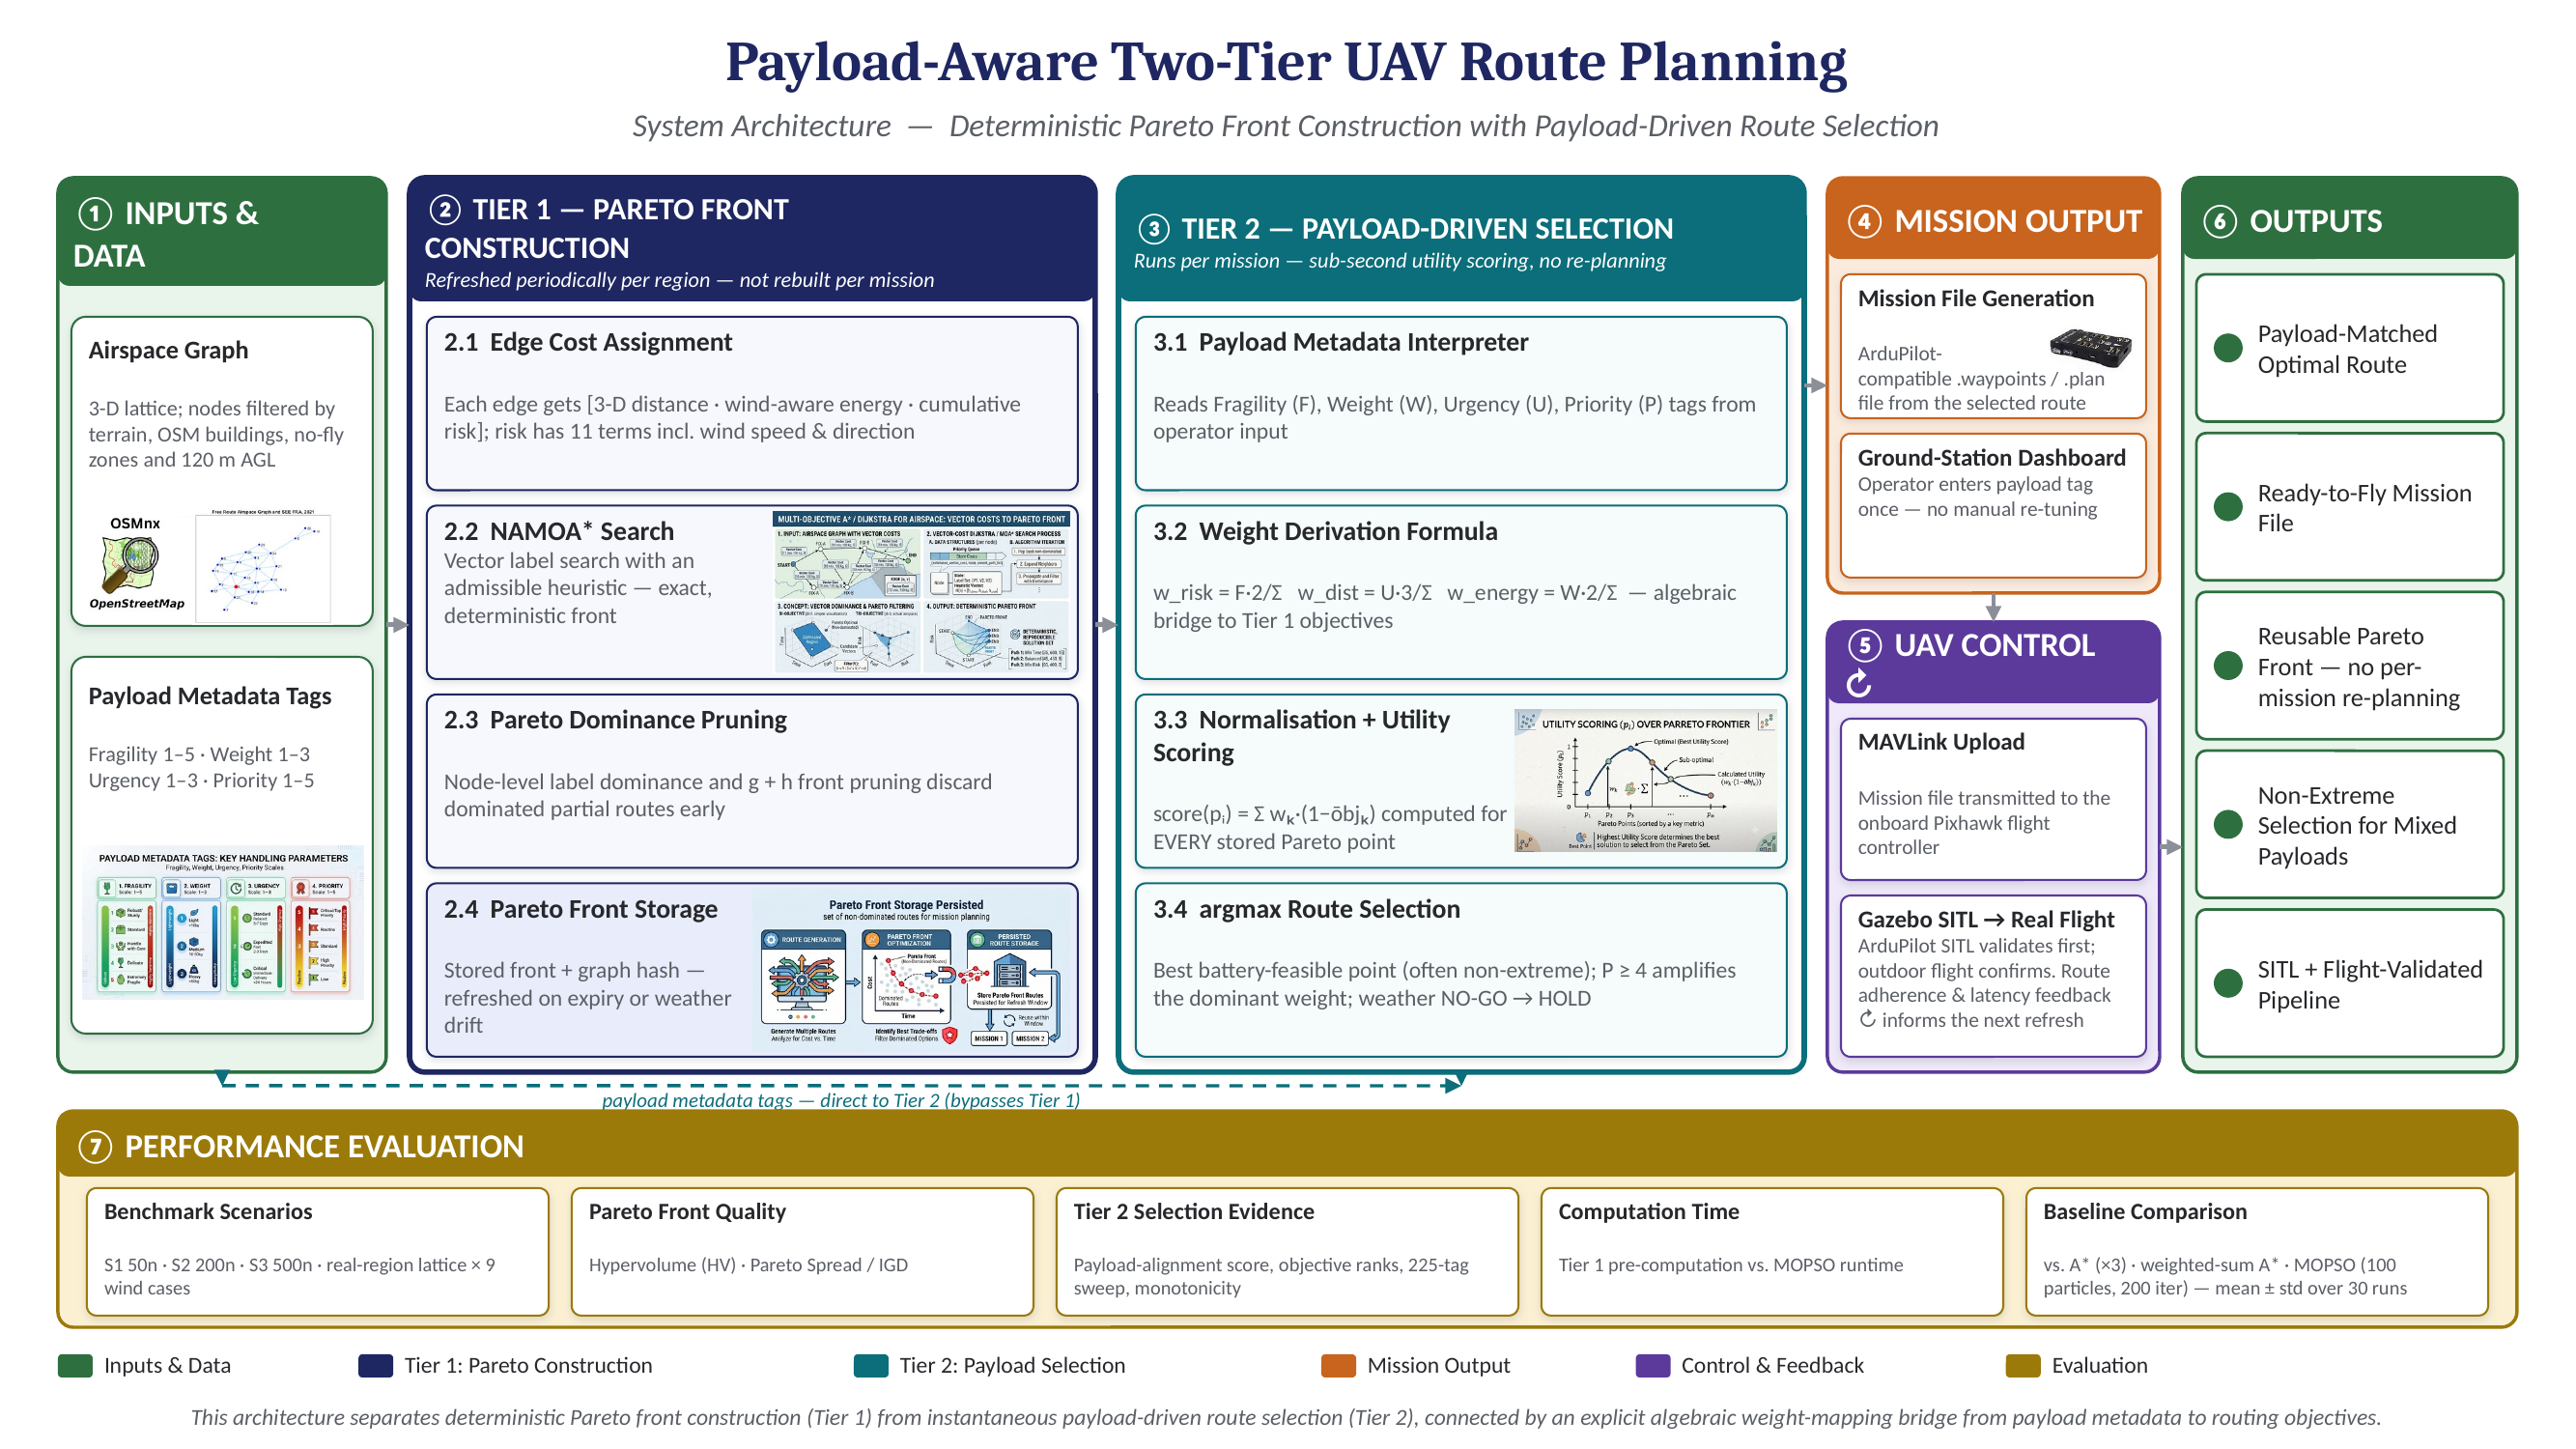
\includegraphics[width=\textwidth]{images/methodology.png}
\caption{Methodology overview: Tier~1 Pareto front construction feeding Tier~2
payload-aware route selection, with mission output, UAV control and evaluation}
\label{fig:methodology}
\end{figure}

\section{ARCHITECTURE DESIGN}\label{sec:arch}

Figure~\ref{fig:architecture} shows the system architecture, which has five layers.
The environment data layer fetches weather, terrain and OpenStreetMap layers and caches
them on disk, so that a network failure falls back to the last good copy instead of
stopping the planner. Module~1 turns these layers into a directed airspace graph whose
edges carry a three-objective cost vector. Tier~1 (Module~2) computes the Pareto front
over that graph and keeps it in a front store, together with what is needed to decide
when it is stale. Tier~2 (Module~4) reads the operator's payload tags and returns one
route from the stored front, or a HOLD advisory when the weather or the battery rules
the mission out. The output layer (Modules~6 and~7) writes the mission file and flies
it in Gazebo with ArduPilot SITL. Modules~3 and~5 sit beside the main path. They run the
baseline planners and compute the quality measures used in Chapter~\ref{cha:results}.

\begin{figure}[!htbp]
\centering
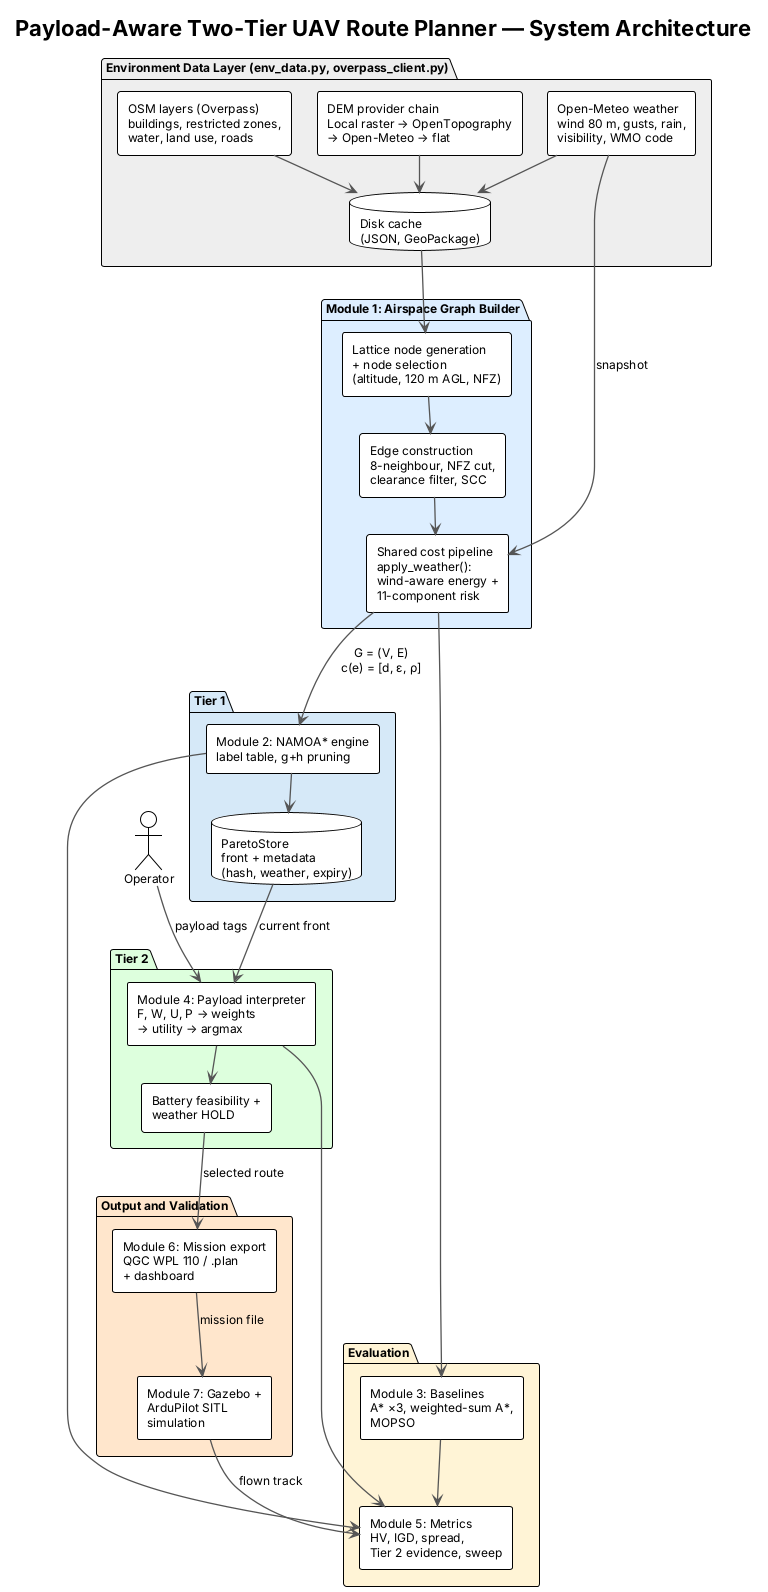
\includegraphics[width=\textwidth,height=0.30\textheight,keepaspectratio]{images/arch.png}
\caption{System architecture. Tier~1 builds and stores the front per region and
weather window; Tier~2 selects a route per payload tag; Modules~6 and~7 export and fly
it}\label{fig:architecture}
\end{figure}

Every edge $e = (u, v)$ of the airspace graph carries the cost vector
\begin{equation}
  \mathbf{c}(e;\omega) = \bigl[d(e),\; \varepsilon(e;\omega),\; \rho(e;\omega)\bigr]
\end{equation}
where $d(e)$ is the three-dimensional length of the segment in kilometres,
$\varepsilon(e;\omega)$ is the wind- and grade-aware energy proxy and $\rho(e;\omega)$
is the cumulative risk exposure along the segment under weather snapshot $\omega$.
Section~\ref{sec:m1} defines all three. The three objectives are to minimise distance,
energy and risk. Route $p$ dominates route $q$, written $p \prec q$, when $p$ is no
worse than $q$ on all three objectives and strictly better on at least one. The Pareto
front $\mathcal{P}$ is the set of routes that no other route dominates.

The code is organised into seven modules. The numbering follows the source files, so
Module~3 holds the baselines and Module~4 holds Tier~2. The sections below describe each
module's purpose, inputs, processing and outputs.

% ------------------------------------------------------------
\section{AIRSPACE GRAPH BUILDER (MODULE 1)}\label{sec:m1}

Module~1 builds the delivery airspace graph $G = (V, E)$. Its inputs are the region
(centre, box size and lattice spacing), the environment layers described below and a
weather snapshot $\omega$. Its output is a directed NetworkX~\cite{r5} graph whose nodes
carry position and altitude and whose edges carry static features, a per-component risk
breakdown and the cost vector $[d, \varepsilon, \rho]$. The weather go/no-go state is
stored on the graph itself so that Tier~2 can read it. Two builders share one cost
pipeline: a lattice builder over a real region, described below, and a seeded synthetic
builder for controlled benchmarks (Section~\ref{sec:dataset}).
Algorithm~\ref{alg:m1} summarises the lattice builder, and the subsections that follow
give the rules behind each step.

\subsection{Environment data acquisition}

Weather comes from the Open-Meteo forecast service~\cite{r20}: the 10\,m wind, gust,
rain, visibility and WMO code, and the hourly 80\,m wind speed and direction. With no
network the last cached snapshot is used, and with no cache the planner assumes calm
air so that runs stay deterministic. Terrain comes from a chain of elevation providers
tried in order (a local GeoTIFF, OpenTopography Copernicus 30\,m, Open-Meteo elevation,
and flat ground as a last resort), each cached on disk. OpenStreetMap buildings,
restricted zones, water and land use are fetched through a multi-endpoint Overpass
client with retries, cached as GeoPackage files~\cite{r4} and indexed in a local metric
frame with Shapely STRtree structures for fast height, distance, containment and
segment-intersection queries.

\subsection{Lattice generation and node selection}

A UAV is not tied to roads, so the airspace is a regular lattice, not a road network.
The region is covered by an $n \times n$ lattice in a local equirectangular frame centred
on the region, with $n = \mathrm{round}(\mathit{box}/\mathit{spacing})$. The default
6\,km box at 200\,m spacing gives 900 candidate nodes. A candidate does not enter the
graph automatically. It has to pass a selection rule that combines four data sources: ground elevation from the DEM, the tallest building in
the node's cell, the legal ceiling and restricted airspace. For node $k$ with ground
elevation $z_k$ and tallest building $b_k$ in its cell,
\begin{equation}
  \mathrm{AGL}_k = \max\bigl(H_\mathrm{cruise},\; b_k + C\bigr), \qquad
  \mathrm{alt}_k = z_k + \mathrm{AGL}_k \label{eq:alt}
\end{equation}
with cruise height $H_\mathrm{cruise} = 60$\,m and clearance $C = 15$\,m. A building's
height is read from its \texttt{height} tag, else from \texttt{building:levels} times
3\,m, else from a default for its type. A node with $\mathrm{AGL}_k > 120$\,m is
blocked, because it cannot be flown legally under the Drone Rules, 2021~\cite{r21}. A
node inside a restricted polygon (an aerodrome, military land, a prison, a protected area
or a government site) is removed. Every surviving node stores its position in both
frames, its ground elevation, the building height, density and mean height of its cell,
its height above ground and its altitude above mean sea level.

\subsection{Edge construction and pruning}

Each surviving node is linked to its eight neighbours in both directions, so the graph
is directed from the start. Three filters then remove edges: any edge whose segment
crosses a restricted polygon, any edge rejected by the optional \texttt{edge\_filter}
hook (used by the simulation module for roof and terrain clearance), and every edge
outside the largest strongly connected component, so that all remaining nodes can reach
each other.

For each edge that survives, the module stores the horizontal haversine length $d_h$,
the forward-azimuth bearing $\theta$, the grade $g = \Delta\mathrm{alt}/d_h$ and the
three-dimensional length $d = \sqrt{d_h^2 + \Delta\mathrm{alt}^2}$.

\subsection{Static risk terms}

Static terms do not depend on the weather, so they are computed once per build. Each
edge is sampled every 25\,m along the straight line between its two endpoint
altitudes. At each sample the module knows the flight altitude, the ground height, the
tallest roof directly below and the tallest roof within 30\,m. Table~\ref{tab:risk} lists all eleven risk components,
static and weather-dependent, with the weight each carries in the edge score
\begin{equation}
  \rho_\mathrm{edge} = \operatorname{clip}\Bigl(\sum_k w_k\,\rho_k,\; 0,\; 1\Bigr),
  \qquad \rho(e;\omega) = \rho_\mathrm{edge}\cdot\frac{d_h}{s} \label{eq:risk}
\end{equation}
where $s$ is the lattice spacing. Multiplying by $d_h/s$ turns the per-edge score into
a cumulative exposure. The risk of a route therefore grows with the distance flown
through risky air.

\begin{small}
\begin{longtable}{|P{2.4cm}|P{10.6cm}|P{1.0cm}|}
\caption{Risk components (every $\rho_k \in [0,1]$) and their weights}\label{tab:risk}\\
\hline
\textbf{Component} & \textbf{Model} & $\boldsymbol{w_k}$\\
\hline
\endfirsthead
\hline
\textbf{Component} & \textbf{Model} & $\boldsymbol{w_k}$\\
\hline
\endhead
Obstacle & Seeded obstacle discs, $0.9(1 - r/R)$ inside a disc (synthetic graphs only) & 1.00\\
\hline
Building & Mean over samples of $[\text{roof within 30\,m}]\cdot\bigl(1-\operatorname{clip}(m/60)\bigr)$, $m$ = margin above that roof & 0.60\\
\hline
Terrain & $\max\bigl(1-\operatorname{clip}(m_{\min}/15),\ \operatorname{clip}(\lvert g\rvert/0.30)\bigr)$: lowest clearance margin or sudden altitude change & 0.30\\
\hline
Wind & $\operatorname{clip}(C\!W/40)$, crosswind against a 40\,km/h saturation speed & 0.30\\
\hline
Gust & $\operatorname{clip}\bigl(0.5\max(0, \mathit{gust} - v)/40\bigr)$ & 0.30\\
\hline
Weather & $0.5\operatorname{clip}(\mathit{rain}/7.5) + 0.5\operatorname{clip}(1 - \mathit{vis}/10\,\mathrm{km})$, uniform over the graph & 0.20\\
\hline
Population & Mean land-use class score along the edge (our values, ranked in the spirit of SORA~\cite{r22}): assembly 1.0, commercial 0.7, major road 0.6, residential 0.5, industrial 0.3 & 0.50\\
\hline
No-fly buffer & $\max_k \exp(-\delta_k/150\,\mathrm{m})$ to the nearest restricted zone, zero beyond 600\,m & 0.80\\
\hline
Water & Fraction of samples over water (risk of losing the payload) & 0.30\\
\hline
Comm/GPS & $\operatorname{clip}(\mathit{density}/0.30)\cdot\operatorname{clip}(\bar{h}/30\,\mathrm{m})$, urban canyon effect & 0.20\\
\hline
Turbulence & $\operatorname{clip}(\mathit{density}/0.30)\cdot\operatorname{clip}(v/40)$ & 0.20\\
\hline
\end{longtable}
\end{small}

The weights are design values that put restricted zones, buildings and crowds ahead of
the weather terms. They have not been calibrated against flight data, and calibrating
them is part of the evaluation work that remains in Phase~I.

\subsection{Wind-aware energy model}

For an edge on bearing $\theta_\mathrm{edge}$ and a wind of speed $v$ blowing from
$\theta_\mathrm{from}$ (the meteorological convention), the headwind and crosswind
components are
\begin{equation}
  H\!W = v\cos(\theta_\mathrm{edge} - \theta_\mathrm{from}), \qquad
  C\!W = v\,\lvert\sin(\theta_\mathrm{edge} - \theta_\mathrm{from})\rvert \label{eq:hwcw}
\end{equation}
A positive $H\!W$ is a headwind. The energy proxy of the edge is
\begin{equation}
  \varepsilon = d\left(1 + \lvert g\rvert + \beta_h\frac{\max(0, H\!W)}{V_c}
  + \beta_c\frac{C\!W}{V_c}\right) \label{eq:energy}
\end{equation}
with cruise airspeed $V_c = 36$\,km/h, $\beta_h = 0.40$ and $\beta_c = 0.15$. A
tailwind earns no credit. This is deliberate: it keeps $\varepsilon \geq d$ on every
edge, and the Tier~1 heuristic relies on that bound. The wind speed is the 80\,m
forecast when available, which is close to the 60--120\,m cruise band. Otherwise the
10\,m value is lifted to cruise height with the power law
\begin{equation}
  v_h = v_{10}\left(\frac{h}{10}\right)^{\alpha}, \qquad \alpha = 0.25
\end{equation}
following Peterson and Hennessey~\cite{r19}. A gust factor measured at 10\,m is applied
to the wind at flight height.

Because of Equation~(\ref{eq:hwcw}), edge costs are directional: flying $u \rightarrow
v$ and $v \rightarrow u$ cost different amounts under wind. This is why the graph is
directed even though the lattice itself is symmetric.

\subsection{Weather-dependent risk and the go/no-go gate}

Four of the eleven risk components change with the weather: crosswind, gust excess,
turbulence and the uniform rain and visibility term. Crosswind depends on the edge
heading, so the same wind makes some corridors riskier than others, and a change of
direction alone can move the low-risk end of the front to a different part of the map.
The function \texttt{apply\_weather(G, $\omega$)} re-costs every edge from its stored
static features, so a new snapshot never requires rebuilding the spatial layers.

The weather gate sits on top of this. A mission is a no-go when the WMO code reports a
thunderstorm (95--99), when rain reaches 7.5\,mm/h, when visibility falls below 1\,km,
or when gusts exceed 45\,km/h, a provisional limit for an F450-class airframe. The
reasons are written to the graph, and Tier~2 refuses to select a route while any reason
is present.

\begin{algorithm}[p]
\caption{Lattice airspace graph construction and costing (Module~1)}\label{alg:m1}
\begin{algorithmic}[1]
\Require Region, box size, spacing $s$; DEM; buildings $\mathcal{B}$; restricted zones $\mathcal{Z}$; weather $\omega$; weights $w_k$; optional \texttt{edge\_filter}
\Ensure Directed graph $G=(V,E)$ with costs $\mathbf{c}(e)=[d,\varepsilon,\rho]$ and no-go reasons $\mathcal{R}$
\State $n \gets \mathrm{round}(\mathit{box}/s)$; place an $n \times n$ lattice in a local equirectangular frame
\For{each lattice point $k$} \Comment{node selection}
  \State $z_k \gets$ DEM elevation; \quad $b_k \gets$ tallest building in the cell of $k$ (from $\mathcal{B}$)
  \State $\mathrm{AGL}_k \gets \max(H_\mathrm{cruise},\, b_k + C)$; \quad $\mathrm{alt}_k \gets z_k + \mathrm{AGL}_k$
  \If{$\mathrm{AGL}_k \leq 120$\,m \textbf{and} $k$ lies outside every polygon in $\mathcal{Z}$} add $k$ to $V$ \EndIf
\EndFor
\For{each $u \in V$ and each of its eight lattice neighbours $v \in V$} \Comment{edge construction}
  \State \textbf{if} segment $uv$ crosses a polygon in $\mathcal{Z}$ \textbf{or} \texttt{edge\_filter}$(u,v)$ rejects it \textbf{then continue}
  \State add the directed edges $(u,v)$ and $(v,u)$ to $E$
\EndFor
\State keep only the largest strongly connected component of $G$
\For{each edge $e=(u,v) \in E$} \Comment{static features and static risk}
  \State $d_h \gets$ haversine length; \quad $\theta \gets$ forward azimuth; \quad $g \gets \Delta\mathrm{alt}/d_h$; \quad $d \gets \sqrt{d_h^2+\Delta\mathrm{alt}^2}$
  \State sample $e$ every 25\,m; read flight altitude, ground height, roof below and roof within 30\,m
  \State store $\rho_k$ for building, terrain, population, no-fly buffer, water and comm/GPS
\EndFor
\State $\mathcal{R} \gets$ reasons among: WMO code 95--99, rain $\geq 7.5$\,mm/h, visibility $< 1$\,km, gust $> 45$\,km/h
\State $v \gets$ 80\,m wind forecast, else $v_{10}(h/10)^{\alpha}$ \Comment{this part re-runs per $\omega$}
\For{each edge $e \in E$}
  \State $H\!W \gets v\cos(\theta-\theta_\mathrm{from})$; \quad $C\!W \gets v\,\lvert\sin(\theta-\theta_\mathrm{from})\rvert$
  \State $\varepsilon \gets d\,\bigl(1+\lvert g\rvert+\beta_h\max(0,H\!W)/V_c+\beta_c\,C\!W/V_c\bigr)$ \Comment{tailwind earns no credit}
  \State compute $\rho_k$ for wind, gust, weather and turbulence
  \State $\rho_\mathrm{edge} \gets \mathrm{clip}\bigl(\sum_k w_k\rho_k,\,0,\,1\bigr)$; \quad $\rho \gets \rho_\mathrm{edge}\,d_h/s$; \quad $\mathbf{c}(e) \gets [d,\varepsilon,\rho]$
\EndFor
\State store $\mathcal{R}$ on $G$; \Return $G$
\end{algorithmic}
\end{algorithm}

% ------------------------------------------------------------
\section{TIER 1 PARETO FRONT ENGINE (MODULE 2)}\label{sec:m2}

Module~2 computes the exact set of non-dominated routes between a source and a target.
Its inputs are the costed graph from Module~1, the two end nodes and an expansion cap.
Its output is the Pareto front $\mathcal{P}$, as a list of cost vectors and node paths,
together with diagnostics: whether the cap truncated the search, how many labels were
expanded and generated, and the runtime.

\subsection{Labels and dominance}

The engine follows NAMOA*~\cite{r17}. Every partial path is a label
$(\mathit{node}, \mathbf{g}, \mathit{parent})$ held in a flat table, and a path is
rebuilt at the end by walking parent ids. Nothing is copied when a label is pushed,
which matters once the label count runs into the thousands. A new label $\mathbf{g}'$ at
node $v$ is discarded if any existing label at $v$ weakly dominates it (is $\leq$ in
every objective, within a small tolerance). Equal vectors count as dominated, so the
front never contains duplicates. Labels that the new one dominates are marked dead and
skipped when popped. No visited set is needed. Every edge has positive distance, so a
path that revisits a node is dominated by its own earlier label at that node, and cycles
die in the dominance check.

\subsection{Admissible vector heuristic and pruning}

The heuristic for node $v$ is
\begin{equation}
  \mathbf{h}(v) = [h,\; h,\; 0]
\end{equation}
where $h$ is the great-circle distance from $v$ to the target. It is admissible for all
three objectives. For distance, every edge has $d \geq d_h$, and the horizontal lengths
of any path to the target add up to at least $h$. For energy,
Equation~(\ref{eq:energy}) gives $\varepsilon \geq d$, so the same bound holds. For
risk, $\rho \geq 0$. A label is pruned when the current front weakly dominates
$\mathbf{g} + \mathbf{h}$. The check is made when the label is generated and again when
it is popped, because the front may have improved in between. The open list is ordered
by $\lVert\mathbf{g} + \mathbf{h}\rVert$, which tends to complete good routes early and
so tightens the pruning sooner.

\subsection{Truncation and front thinning}

An expansion cap protects the planner from a runaway search. When the cap is hit, the
result is flagged as truncated only if some live label could still improve the front.
An optional $\varepsilon$-dominance step can cap very large fronts at $N$ routes while
keeping the three single-objective extremes; it is off by default, so the benchmarks
use the exact front.

Algorithm~\ref{alg:tier1} gives the full procedure. Here $\preceq$ is weak dominance.

\begin{algorithm}[p]
\setstretch{1.58}% stretched to fill the page
\caption{NAMOA* with a label table (Tier~1)}\label{alg:tier1}
\begin{algorithmic}[1]
\Require Graph $G=(V,E)$, source $s$, target $t$, costs $\mathbf{c}(u,v)=[d,\varepsilon,\rho]$, cap $M$
\Ensure Pareto front $\mathcal{P}$, flag $\mathit{truncated}$
\State $L \gets [(s, [0,0,0], -1)]$; $\mathit{at}[s] \gets \{0\}$; $F \gets \emptyset$; $\mathit{Open} \gets \{(\lVert\mathbf{h}(s)\rVert, 0)\}$
\While{$\mathit{Open} \neq \emptyset$}
  \If{$\mathit{expanded} \geq M$}
    \State $\mathit{truncated} \gets \exists$ live $\ell \in \mathit{Open}$ with $F \not\preceq \mathbf{g}_\ell + \mathbf{h}(u_\ell)$; \textbf{break}
  \EndIf
  \State $\ell = (u, \mathbf{g}) \gets$ \Call{PopMin}{$\mathit{Open}$}
  \State \textbf{if} $\ell$ is dead \textbf{or} $F \preceq \mathbf{g} + \mathbf{h}(u)$ \textbf{then continue}
  \State $\mathit{expanded} \gets \mathit{expanded} + 1$
  \For{each successor $v$ of $u$}
    \State $\mathbf{g}' \gets \mathbf{g} + \mathbf{c}(u,v)$
    \State \textbf{if} $\exists\, o \in \mathit{at}[v] : \mathbf{g}_o \preceq \mathbf{g}'$ \textbf{then continue} \Comment{node dominance}
    \State \textbf{if} $F \preceq \mathbf{g}' + \mathbf{h}(v)$ \textbf{then continue} \Comment{prune on $g+h$}
    \State mark dead every $o \in \mathit{at}[v]$ with $\mathbf{g}' \preceq \mathbf{g}_o$
    \State append label $(v, \mathbf{g}', \ell)$ to $L$ and to $\mathit{at}[v]$
    \If{$v = t$}
      \State $F \gets \{f \in F : \mathbf{g}' \not\preceq f\} \cup \{\mathbf{g}'\}$
    \Else
      \State push $(\lVert\mathbf{g}' + \mathbf{h}(v)\rVert, \text{label})$ onto $\mathit{Open}$
    \EndIf
  \EndFor
\EndWhile
\State rebuild each route in $F$ by following parent ids; \Return $\mathcal{P}$, $\mathit{truncated}$
\end{algorithmic}
\end{algorithm}

\subsection{Why an exact method}

A population method is usually faster on a large graph. We chose an exact search because
the same graph and weather always give the same front, because the interior routes that
mixed payloads need are the ones a stochastic archive tends to miss
(Section~\ref{sec:perf-front}), and because Tier~1 runs only once per region and weather
window.

\subsection{Pareto front store and refresh}

The front is reused across missions, so the system needs a rule for when reuse is safe.
The front store saves one JSON record per (region, source, target) with the front, a
SHA-256 hash of the static graph (never the weather-dependent costs), the weather
snapshot it was built for, a validity limit three hours after creation, the truncation
flag and the search diagnostics.

On each request the store lists the reasons the record cannot be reused
: no record, a forced refresh, a different static graph, a
different identity, expiry, or weather drift. Drift means the wind speed has moved by
more than 10\,km/h, the direction has turned by more than 45$^\circ$ while the wind is
above 10\,km/h, the gust has moved by more than 15\,km/h, or the go/no-go state has
flipped. With no reason, Tier~2 runs against the stored front and no search happens.
With a reason, only \texttt{apply\_weather} and Tier~1 run again, and the spatial layers
stay cached.

% ------------------------------------------------------------
\section{BASELINE PLANNERS (MODULE 3)}\label{sec:m3}

Module~3 holds the planners that Tier~1 and Tier~2 are compared against. They read the
same costed graph, so any difference in the results comes from the search method and
not from the data.

Three single-objective A* searches minimise distance, energy and risk separately; the
distance search uses the haversine heuristic and the other two a zero heuristic. Each
returns one extreme point of the front. A weighted-sum A* scalarises the cost vector
with a preset's Tier~2 weights, $c_w(e) = \sum_j w_j c_j(e)/s_j$, where $s_j$ is the
spread of objective $j$ across the three extreme routes. This is the classic approach
our problem statement criticises, and it can reach only supported points on the convex
hull of the front. The population baseline adapts MOPSO~\cite{r6} to graph routes: a
particle is a valid path, the swarm is seeded with the extreme routes and biased random
walks, and in each iteration a particle follows its personal best or an archive leader
for part of the way and is repaired to the target with a weighted shortest suffix. The
archive uses the same dominance helper as Tier~1. Report-scale settings are 100
particles, 200 iterations, an archive of 100 and 30 seeded repetitions.

% ------------------------------------------------------------
\section{TIER 2 PAYLOAD METADATA INTERPRETER (MODULE 4)}\label{sec:m4}

Module~4 turns a description of the payload into a route. Its inputs are the stored
front, the weather go/no-go reasons from the graph and the four tags
$(F, W, U, P_\mathrm{lvl})$. Its output is a selection record: the tags, the derived
weights, the selected route's index, cost vector and waypoints, the normalised scores,
its rank on each objective, whether it is an extreme or non-extreme point, the latency,
the number of battery-feasible routes and, when no route can be flown, a HOLD advisory.
The record is written to JSON and CSV. A tag outside its integer range raises an error
before any weight is derived, so a typing mistake cannot quietly change the route.

\subsection{Semantic mapping}

The bridge between the tiers maps each payload tag to exactly one Tier~1 objective, as
Table~\ref{tab:semantic-mapping} shows.

\begin{table}[!htbp]
\centering
\caption{Semantic mapping from payload tags to Tier~1 objectives}\label{tab:semantic-mapping}
\small
\begin{tabular}{|P{3.0cm}|P{1.2cm}|P{3.6cm}|P{6.2cm}|}
\hline
\textbf{Payload tag} & \textbf{Range} & \textbf{Tier~1 objective} & \textbf{Reasoning}\\
\hline
Fragility class $F$ & 1--5 & $w_\mathrm{risk}$ (flight risk) & Fragile items should avoid turbulent, exposed and crowded corridors\\
\hline
Payload weight class $W$ & 1--3 & $w_\mathrm{energy}$ (energy) & A heavier payload raises hover and lift power, so energy matters more\\
\hline
Delivery urgency $U$ & 1--3 & $w_\mathrm{dist}$ (distance) & Time-critical deliveries need the shortest path\\
\hline
Priority level $P_\mathrm{lvl}$ & 1--5 & Amplifier & Strengthens the dominant weight for high-priority missions\\
\hline
\end{tabular}
\end{table}

\subsection{Weight derivation}

From the tags, three weights are derived with no expert input:
\begin{align}
  r_\mathrm{raw} &= 2F, \qquad d_\mathrm{raw} = 3U, \qquad e_\mathrm{raw} = 2W,
  \qquad S = r_\mathrm{raw} + d_\mathrm{raw} + e_\mathrm{raw} \label{eq:raw}\\
  w_\mathrm{risk} &= \frac{r_\mathrm{raw}}{S}, \qquad
  w_\mathrm{dist} = \frac{d_\mathrm{raw}}{S}, \qquad
  w_\mathrm{energy} = \frac{e_\mathrm{raw}}{S} \label{eq:weights}
\end{align}
The multipliers (2 for fragility and payload weight, 3 for urgency) encode the
assumption that, in medical delivery, urgency is more sensitive than fragility or
payload weight. Payload weight is tied to energy because a heavier payload directly
raises the power needed to hover and climb. No such direct physical link exists to risk
or to distance.

Every weight depends on all three raw scores. Raising $F$ raises $w_\mathrm{risk}$ and
lowers the other two at the same time, so one tag change moves the whole weight vector.
This is the reason the formula is not a lookup table. There is no fixed list of payload
types, and any of the $5 \times 3 \times 3 \times 5 = 225$ tag combinations gives a
valid, different weighting.

For high-priority missions ($P_\mathrm{lvl} \geq 4$), the largest weight is amplified:
\begin{equation}
  w_\mathrm{max} \leftarrow w_\mathrm{max} + 0.1\,w_\mathrm{max}, \qquad
  w_j \leftarrow \frac{w_j}{\sum_k w_k} \label{eq:amplify}
\end{equation}
A flat bonus added to every score was rejected, because it never changes which route
scores highest.

\subsection{Utility scoring and selection}

For each Pareto point $p_i$ with objective values $(d_i, \varepsilon_i, \rho_i)$, the
values are min-max normalised over the whole front,
\begin{equation}
  \tilde{d}_i = \frac{d_i - d_{\min}}{d_{\max} - d_{\min}}, \quad
  \tilde{\varepsilon}_i = \frac{\varepsilon_i - \varepsilon_{\min}}{\varepsilon_{\max} - \varepsilon_{\min}}, \quad
  \tilde{\rho}_i = \frac{\rho_i - \rho_{\min}}{\rho_{\max} - \rho_{\min}}
\end{equation}
so that 0 is the best value on the front and 1 the worst. A degenerate objective, where
all routes are equal, normalises to zero. The utility score is
\begin{equation}
  \mathrm{score}(p_i) = w_\mathrm{dist}(1 - \tilde{d}_i) + w_\mathrm{energy}(1 - \tilde{\varepsilon}_i) + w_\mathrm{risk}(1 - \tilde{\rho}_i) \label{eq:score}
\end{equation}
and the mission route is $p^* = \arg\max_{p_i \in \mathcal{P}} \mathrm{score}(p_i)$.
Ties go to the lower index, so the result is deterministic.

The argmax runs over the full front, so Tier~2 can land anywhere on it, including
between the extremes. For a payload with mixed needs the best-scoring
route is often an interior one that no single-objective search would return.

\subsection{Reference presets}

Table~\ref{tab:presets} gives the weights the formula produces for four reference
presets. Only emergency medicine has $P_\mathrm{lvl} \geq 4$, so it is the only preset
whose dominant weight is amplified.

\begin{table}[!htbp]
\centering
\caption{Reference payload presets and their derived weights}\label{tab:presets}
\small
\begin{tabular}{|l|c|c|c|c|c|c|c|}
\hline
\textbf{Preset} & $F$ & $W$ & $U$ & $P_\mathrm{lvl}$ & $w_\mathrm{risk}$ & $w_\mathrm{dist}$ & $w_\mathrm{energy}$\\
\hline
Fragile medical sample & 5 & 1 & 1 & 3 & 0.667 & 0.200 & 0.133\\
\hline
Emergency medicine & 1 & 1 & 3 & 5 & 0.144 & 0.712 & 0.144\\
\hline
Disaster relief & 1 & 3 & 1 & 2 & 0.182 & 0.273 & 0.545\\
\hline
Mixed cargo & 3 & 2 & 2 & 3 & 0.375 & 0.375 & 0.250\\
\hline
\end{tabular}
\end{table}

As a worked example, take emergency medicine. The raw scores are $r_\mathrm{raw} = 2$,
$d_\mathrm{raw} = 9$ and $e_\mathrm{raw} = 2$, which sum to 13, so the weights before
amplification are $0.154$, $0.692$ and $0.154$. The priority is 5, so the distance
weight grows by a tenth to $0.762$. After renormalising by the new total of $1.069$, the
weights are $w_\mathrm{risk} = 0.144$, $w_\mathrm{dist} = 0.712$ and
$w_\mathrm{energy} = 0.144$, which are the values in the table.

\subsection{Battery feasibility}

The payload weight class also decides whether a route can be flown at all. Each class
maps to a nominal payload mass $m_W$ (0.25, 0.5 and 1.0\,kg for $W = 1, 2, 3$), and a
route's energy proxy is converted to watt-hours with
\begin{equation}
  E_\mathrm{Wh} = k_\mathrm{cal}\,\varepsilon\left(\frac{m_\mathrm{uav} + m_W}{m_\mathrm{uav}}\right)^{1.5} \label{eq:battery}
\end{equation}
where the exponent follows the way induced rotor power scales with weight. With the
current values ($k_\mathrm{cal} = 6$\,Wh per unit of energy proxy,
$m_\mathrm{uav} = 1.5$\,kg, a 74\,Wh battery and a 20\% reserve), a route is feasible
when it needs at most 59.2\,Wh. Infeasible routes are removed before the argmax. These
constants are marked as placeholders in the code and will be replaced by values
calibrated in simulation.

\subsection{Weather hold and decision record}

If the weather gate reports any reason, or if no route on the front is battery-feasible,
Tier~2 returns a HOLD advisory that says why, instead of a route. Otherwise it returns
the feasible route with the highest score.

Algorithm~\ref{alg:tier2} gives the full procedure. No search runs at this stage. The
cost is one pass over the stored front, so the latency is a few milliseconds.

\begin{algorithm}[p]
\setstretch{1.07}% stretched to fill the page
\caption{Payload-aware route selection on the stored front (Tier~2)}\label{alg:tier2}
\begin{algorithmic}[1]
\Require Front $\mathcal{P}=\{(\mathbf{c}_i,\pi_i)\}_{i=1}^{K}$, $\mathbf{c}_i=[d_i,\varepsilon_i,\rho_i]$; no-go reasons $\mathcal{R}$; tags $(F,W,U,P_\mathrm{lvl})$; $m_W$, $m_\mathrm{uav}$, $k_\mathrm{cal}$, $E_\mathrm{bat}$, reserve $\eta$
\Ensure Mission route $\pi^*$ and its selection record, or a HOLD advisory
\State \textbf{if} $F, P_\mathrm{lvl} \notin \{1,\ldots,5\}$ \textbf{or} $W, U \notin \{1,2,3\}$ \textbf{then raise} an error \Comment{before any weight is derived}
\State $r_\mathrm{raw} \gets 2F$; \quad $d_\mathrm{raw} \gets 3U$; \quad $e_\mathrm{raw} \gets 2W$; \quad $S \gets r_\mathrm{raw}+d_\mathrm{raw}+e_\mathrm{raw}$
\State $w_\mathrm{risk} \gets r_\mathrm{raw}/S$; \quad $w_\mathrm{dist} \gets d_\mathrm{raw}/S$; \quad $w_\mathrm{energy} \gets e_\mathrm{raw}/S$
\If{$P_\mathrm{lvl} \geq 4$} \Comment{priority amplifier}
  \State $w_\mathrm{max} \gets 1.1\,w_\mathrm{max}$ for the largest of the three weights
  \State divide every weight by $w_\mathrm{risk}+w_\mathrm{dist}+w_\mathrm{energy}$
\EndIf
\For{each objective $j \in \{d,\varepsilon,\rho\}$} \Comment{front-wide ranges}
  \State $\mathit{lo}_j \gets \min_i c_{i,j}$; \quad $\mathit{hi}_j \gets \max_i c_{i,j}$
\EndFor
\State $E_\mathrm{use} \gets E_\mathrm{bat}(1-\eta)$; \quad $\mathcal{F} \gets \emptyset$
\For{$i = 1$ \textbf{to} $K$}
  \For{each objective $j$} \Comment{min--max normalisation}
    \State $\tilde{c}_{i,j} \gets 0$ if $\mathit{hi}_j = \mathit{lo}_j$, else $(c_{i,j}-\mathit{lo}_j)/(\mathit{hi}_j-\mathit{lo}_j)$
  \EndFor
  \State $s_i \gets w_\mathrm{dist}(1-\tilde{d}_i) + w_\mathrm{energy}(1-\tilde{\varepsilon}_i) + w_\mathrm{risk}(1-\tilde{\rho}_i)$
  \State $E_{\mathrm{Wh},i} \gets k_\mathrm{cal}\,\varepsilon_i\,\big((m_\mathrm{uav}+m_W)/m_\mathrm{uav}\big)^{1.5}$ \Comment{battery proxy}
  \If{$E_{\mathrm{Wh},i} \leq E_\mathrm{use}$} $\mathcal{F} \gets \mathcal{F} \cup \{i\}$ \EndIf
\EndFor
\If{$\mathcal{R} \neq \emptyset$}
  \State \Return HOLD, with the weather reasons in $\mathcal{R}$
\ElsIf{$\mathcal{F} = \emptyset$}
  \State \Return HOLD, no route fits $E_\mathrm{use}$ at payload class $W$
\EndIf
\State $i^* \gets \arg\max_{i \in \mathcal{F}} s_i$, ties to the lower index \Comment{full front, not only extremes}
\State $\mathit{rank}_j \gets$ position of $c_{i^*,j}$ among the sorted values of objective $j$
\State $\mathit{type} \gets$ \textit{extreme} if $i^*$ is best on any objective, else \textit{non-extreme}
\State $\mathit{wp} \gets$ (latitude, longitude, altitude) of every node on $\pi_{i^*}$
\State write tags, weights, $i^*$, $\mathbf{c}_{i^*}$, $\mathit{wp}$, $\mathbf{s}$, $\mathit{rank}$, $\mathit{type}$, $|\mathcal{F}|$ and latency to JSON and CSV
\State \Return $\pi_{i^*}$ and the selection record
\end{algorithmic}
\end{algorithm}

% ------------------------------------------------------------
\section{EVALUATION AND BENCHMARKING (MODULE 5)}\label{sec:m5}

Module~5 measures how good a front is and how sensible the Tier~2 picks are. Every
measure is computed per scenario, and the results are written to CSV and JSON so that
each pass of the evaluation can be compared with the previous one.

\subsection{Front quality measures}

There is no known true front for our graphs, so the reference front $\mathcal{R}$ of a
scenario is the non-dominated union of every route found by every method and
repetition, and all measures are computed in the space normalised by its ideal and
nadir points. The hypervolume (HV)~\cite{r18} is the volume dominated by a front and bounded by a
reference point, here the normalised nadir padded by 10\%, $[1.1, 1.1, 1.1]$. It is
computed exactly in three dimensions by slicing along the first objective and solving
the two-dimensional problem on each slice. Larger is better. The inverted generational
distance (IGD) measures how well a front $A$ covers the reference front:
\begin{equation}
  \mathrm{IGD}(A, \mathcal{R}) = \frac{1}{\lvert\mathcal{R}\rvert}\sum_{r \in \mathcal{R}} \min_{a \in A} \lVert r - a \rVert_2
\end{equation}
Smaller is better, and zero means that $A$ contains every reference point. The spread
$\Delta$ measures how evenly the points are distributed and how far they reach toward
the extremes of $\mathcal{R}$; smaller is better. Runtime and front size are recorded
for every method.

\subsection{Tier 2 evidence}

We do not report a Tier~2 ``accuracy'', because there is no ground-truth label that
says which route is correct for a payload. For each preset the module records the
selected route's rank on each objective, whether it is an extreme or non-extreme point,
the latency, and a rank-based payload-alignment score
\begin{equation}
  A = \sum_{k \in \{d, \varepsilon, \rho\}} w_k\left(1 - \frac{\mathrm{rank}_k - 1}{K - 1}\right)
\end{equation}
where $K$ is the front size. Because $A$ uses ranks, it does not depend on the min-max
utility that Tier~2 itself maximises. The same score is computed for four competing
selection rules on the same front: the shortest route, the knee point (the point
farthest from the line joining the distance and risk extremes), the largest NSGA-II
crowding distance~\cite{r8,r3}, and a fixed equal-weight utility in the style
of~\cite{r1}.

\subsection{Tag sweep and monotonicity}

A sweep runs Tier~2 for all 225 tag combinations. It counts distinct selected routes
and non-extreme picks, and it checks monotonicity: raising $F$ with the other tags
fixed must never raise the selected route's risk, raising $U$ must never raise its
distance, and raising $W$ must never raise its energy. The target is zero violations.

\subsection{The evaluation cycle}

Benchmarking is a repeated cycle, not a single run: fix the scenarios, run every method,
score the fronts, check the Tier~2 picks, fly the routes in simulation, analyse the weak
spots, change the model and run everything again. One full pass covers four graphs
under nine wind cases with MOPSO at 100 particles, 200 iterations and 30 repetitions,
about 21.6 million particle updates in all.

% ------------------------------------------------------------
\section{MISSION EXPORT AND DASHBOARD (MODULE 6)}\label{sec:m6}

\subsection{Mission file generation}

Module~6 writes the selected route as a QGC WPL~110 file and a QGroundControl
\texttt{.plan} file, merging consecutive waypoints that keep the same bearing and slope.
Route waypoints use frame~3 (\texttt{GLOBAL\_RELATIVE\_ALT}), measured from home, so
the exporter writes
\begin{equation}
  \mathit{alt}_\mathrm{rel} = \mathit{alt}_\mathrm{AMSL} - H_\mathrm{home}
\end{equation}
with $H_\mathrm{home}$ the ground elevation under the first waypoint. The height above
the local ground is never written into frame~3, because that would be wrong wherever
the terrain varies.

\subsection{Operator dashboard}

A small Tkinter dashboard lets an operator load a stored graph and front, type the four
tags, see the route on a map and export the mission. Two defects are open: it does not
yet pass the weather reasons to Tier~2, and it can load a graph and a front from
different runs.

% ------------------------------------------------------------
\section{SIMULATION AND SITL VALIDATION (MODULE 7)}\label{sec:m7}

A route that scores well on the graph may still be hard to fly, so Module~7 checks the
flight itself. It flies the Tier~2 route through a three-dimensional model of the
delivery area in Gazebo Harmonic~\cite{r24}, with ArduCopter running in
software-in-the-loop~\cite{r23}, and compares the flown track with the plan.
Communication with the autopilot uses MAVLink~\cite{r7}. The simulation code imports the
planner modules directly; nothing is copied. Figure~\ref{fig:sim} shows the pipeline.

\begin{figure}[!htbp]
\centering
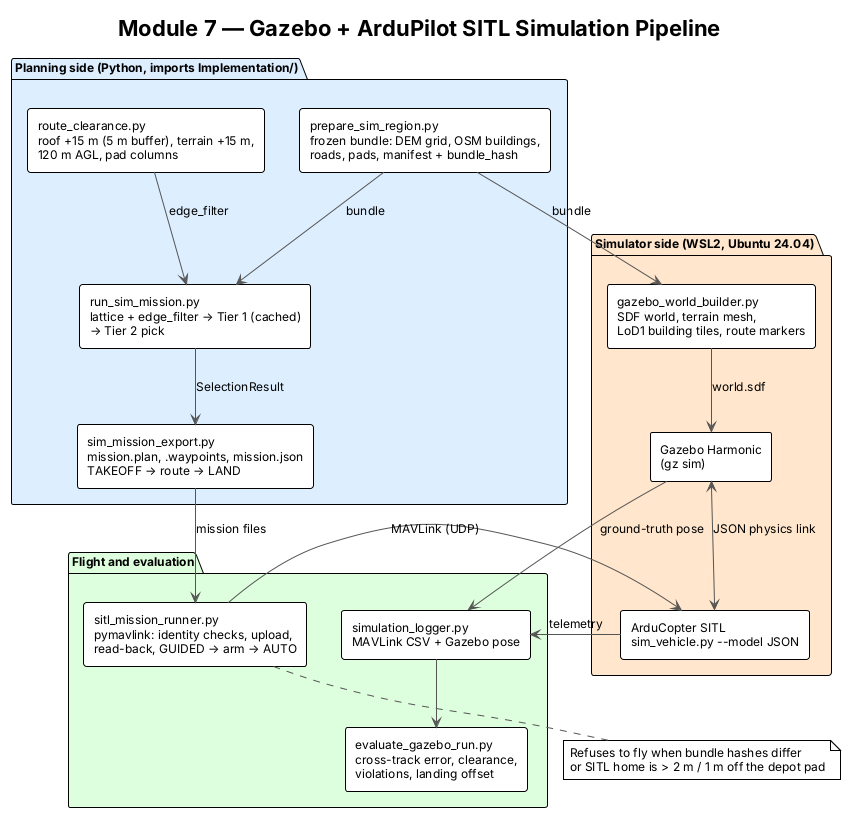
\includegraphics[width=\textwidth,height=0.28\textheight,keepaspectratio]{images/simulation.png}
\caption{Gazebo and ArduPilot SITL simulation pipeline}\label{fig:sim}
\end{figure}

\subsection{Bundle, clearance and frame contract}

A region is first frozen into a bundle: a terrain grid, OSM buildings with heights,
roads, the depot and destination pads, and a manifest. Its hash is written into the
graph, the front, the mission file and the world, and the runner refuses to fly if they
do not match. Before NAMOA* runs, a clearance checker passed in as \texttt{edge\_filter}
removes every edge that passes less than 15\,m above a buffered roof or the terrain, or
goes above 120\,m above ground. The Gazebo world has its origin at the depot pad, where
SITL also places home, so a mission altitude means the same height in the planner, the
world and the autopilot.

\subsection{Mission sequence}

Figure~\ref{fig:sequence} follows one mission from the operator's tags to the flown
route. Tier~1 runs only when the stored front is stale or missing. Tier~2 then returns
either a HOLD advisory or a selection that is exported as a mission file. The runner uploads and reads back the mission, arms, switches to AUTO and
logs telemetry until landing. An evaluator then computes the cross-track error, the
minimum clearance, any rule breach and the landing offset from the pad.

\begin{figure}[!htbp]
\centering
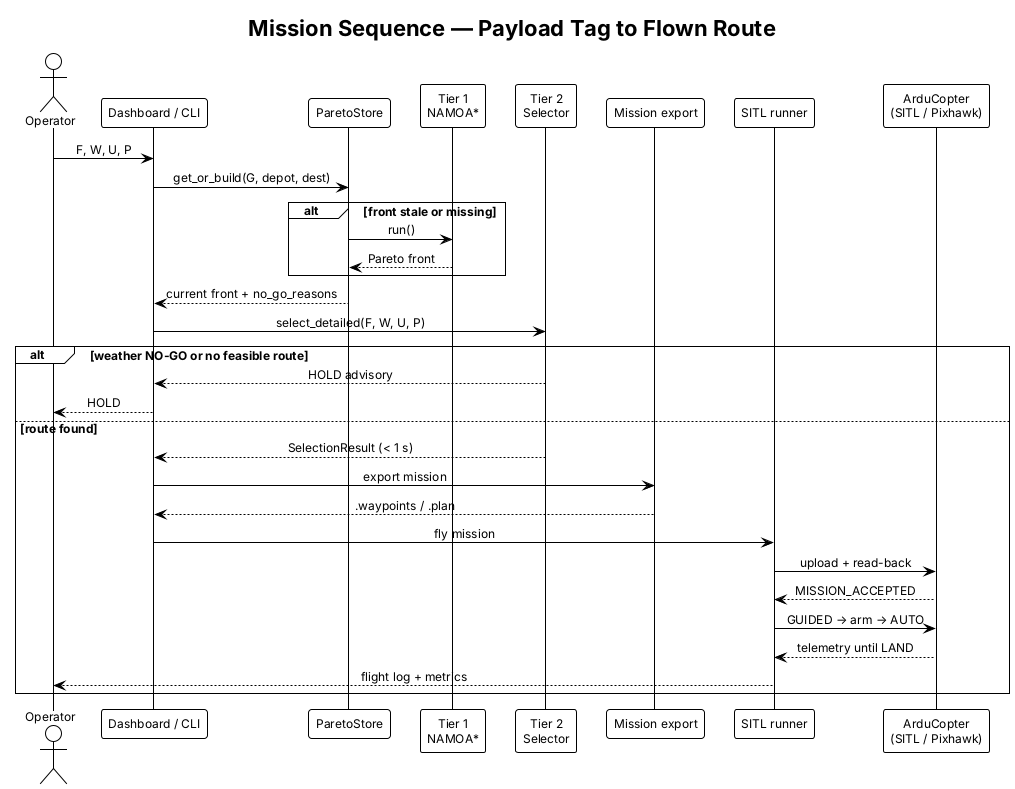
\includegraphics[width=0.72\textwidth]{images/mission_sequence.png}
\caption{Mission sequence from payload tag entry to the flown route}\label{fig:sequence}
\end{figure}
 % PROPOSED METHODOLOGY
% Chapter 4

\chapter{EXPERIMENTAL RESULTS AND PERFORMANCE ANALYSIS}\label{cha:results}

This chapter contains the information that forms the basis of the system, both the
hardware and software, the experiments carried out thus far, and the conclusions made
from them. The quantitative results come from four different places: the first run of
the evaluation loop (refer Section~\ref{sec:m5}), wind experiment, the ablation runner,
and the very first SITL flights. They are
preliminary in a specific sense: MOPSO was run at reduced settings, the risk weights and
battery constants are not yet calibrated, and the synthetic density labels have a known
defect. Each caveat is stated next to the result it affects.

\section{DATASET DESCRIPTION}\label{sec:dataset}

The datasets of the works we reviewed are custom or not released, so, as is common in
this field, we built our own environments. There are two kinds: synthetic airspace graphs, generated from fixed seeds, for
controlled benchmarks; and a real-region lattice built from public geographic and
weather data. Table~\ref{tab:datasets} lists every graph used in this chapter.

\begin{table}[!htbp]
\centering
\caption{Graphs and scenarios used in the experiments}\label{tab:datasets}
\small
\begin{tabular}{|P{3.0cm}|P{2.9cm}|P{8.3cm}|}
\hline
\textbf{Scenario} & \textbf{Size} & \textbf{Description}\\
\hline
S1 small sparse & 50 nodes & Synthetic grid, seed 101, 5\% obstacle coverage label, weather seeded\\
\hline
S2 medium & 196--200 nodes & Synthetic grid, seed 202, 20\% label; weather seeded (benchmark) or set explicitly (wind experiment)\\
\hline
S3 large dense & 500 nodes & Synthetic grid, seed 303, 40\% label, weather seeded\\
\hline
Real-region lattice & 893 nodes, 6,752 edges & 6\,km box, 200\,m spacing, offline fixture layers (ablation)\\
\hline
Small lattice & 2\,km box, 200\,m spacing & Lattice used for the route figure in Section~\ref{sec:perf-tier2}\\
\hline
Flat lattice & 225 nodes, 1,624 edges & 3\,km box, 200\,m spacing, no layers (directional cost check)\\
\hline
Simulation bundle & 1.5\,km box, 100\,m lattice & Frozen terrain, buildings, roads and pads for Gazebo and SITL\\
\hline
\end{tabular}
\end{table}

\subsection{Synthetic airspace graphs}

The synthetic graphs come from the seeded builder of Section~\ref{sec:m1}. Each is a
jittered grid of about 1.3\,km spacing with 8-neighbour directed edges, seeded Gaussian
hills for terrain, obstacle discs, and seeded wind between 12 and 28\,km/h with a gust
factor of 1.4. The three scales (50, 200 and 500 nodes) were chosen to cover a sanity
check, a mid-sized core case and a stress case. Every draw comes from the seed, so the graphs are reproducible.

There is one known defect in this data. The density obstacle labels (5\%, 20\% and
40\%) do not affect the graph builder at all; rather, the benchmark runner rescales the
end risk value. As a result, the scenarios vary in size and seeds and not in obstacle
density regardless of the labels. This is corrected in the next pass, and all benchmark
values are recalculated.

\subsection{Real-region lattice}

Four public data sources feed the real-region lattice (Table~\ref{tab:sources}).
Nothing in the method ties it to one place; our example is a coastal urban
neighbourhood. The default 6\,km box at 200\,m spacing has 900 candidate nodes, of which 893 remain after node selection and connectivity pruning in the fixture run, linked by
6,752 directed edges.

\begin{table}[!htbp]
\centering
\caption{Environment data sources for the real-region lattice}\label{tab:sources}
\small
\begin{tabular}{|P{2.8cm}|P{4.3cm}|P{7.1cm}|}
\hline
\textbf{Layer} & \textbf{Source} & \textbf{Used for}\\
\hline
Weather & Open-Meteo forecast~\cite{r20} & Wind speed and direction at 10\,m and 80\,m, gust, rain, visibility, WMO code\\
\hline
Terrain & Local GeoTIFF, OpenTopography Copernicus 30\,m, Open-Meteo elevation (Copernicus 90\,m), flat fallback & Ground elevation of nodes and edge samples\\
\hline
Buildings & OpenStreetMap via Overpass & Footprints and heights; node altitude, building risk, density, turbulence, urban canyon\\
\hline
Restricted zones & OpenStreetMap via Overpass & Aerodromes, military land, prisons, protected areas, government sites; node and edge removal, soft buffer\\
\hline
Water and land use & OpenStreetMap via Overpass, coastline & Water fraction, population exposure classes, major roads\\
\hline
\end{tabular}
\end{table}

Public Overpass server sometimes resets or times out. For the offline and replicable
experiments, the project offers fixture layers that represent manually created test data
mimicking the real region. The ablation from Section~\ref{sec:perf-ablation} was done
using such fixtures showing how each layer affects the planner rather than providing
metrics available in reality.

\subsection{Payload tag space and simulation bundle}

We evaluate Tier~2 on all 225 tag combinations. Four reference presets
(Table~\ref{tab:presets}) stand in for deliveries led by risk, by distance and by
energy, and one balanced delivery. For simulation we freeze a 1.5\,km region into a
bundle, and its hash binds the planner graph, stored front, mission file and Gazebo
world to each other.

\section{ECOSYSTEM}\label{sec:ecosystem}

\subsection{Hardware configuration}

All planner experiments in this chapter ran on a laptop-class CPU without a GPU. The
planner does not need one: Tier~1 is a graph search that runs on a single core, and
Tier~2 is a closed-form computation. The simulation runs under WSL2 (Ubuntu 24.04) on
the same class of machine.

Phase~II moves the system onto standard, commercially available hardware: an F450
quadcopter frame with a Pixhawk flight controller running ArduCopter, a Raspberry Pi~5
companion computer that hosts Tier~2 on board, a servo payload release and a MAVLink
telemetry link to the ground station.

\subsection{Software environment}

All code is written in Python~3. NetworkX~\cite{r5} holds the directed airspace
graph and runs the A* baselines; NumPy handles dominance checks and metrics; Shapely~2
STRtree indexes hold the spatial layers; and GeoPandas, pyogrio and OSMnx~\cite{r4}
parse and cache the OpenStreetMap layers. Figures use Matplotlib, the dashboard
Tkinter, and the offline test suites unittest. Simulation uses Gazebo
Harmonic~\cite{r24}, ArduPilot SITL~\cite{r23}, pymavlink over MAVLink~\cite{r7} and
QGroundControl.

\section{EXPERIMENTS CONDUCTED}\label{sec:experiments}

Table~\ref{tab:experiments} summarises the experiments. Each is described below, and
Section~\ref{sec:performance} analyses the results.

\begin{table}[!htbp]
\centering
\caption{Experiments carried out in Phase~I so far}\label{tab:experiments}
\small
\begin{tabular}{|P{0.7cm}|P{3.5cm}|P{3.2cm}|P{6.6cm}|}
\hline
\textbf{No.} & \textbf{Experiment} & \textbf{Data} & \textbf{Question}\\
\hline
E1 & Front quality benchmark & S1, S2, S3 & Does the exact Tier~1 front beat single-objective A* and MOPSO on HV, IGD and spread, and at what runtime cost?\\
\hline
E2 & Wind direction study & S2 under calm air and 8 directions; 15$^\circ$ sweep & How much does wind direction alone change the front and the Tier~2 picks?\\
\hline
E3 & Directional edge costs & Flat lattice, wind from the east & Do edge costs respond to heading as the model predicts?\\
\hline
E4 & Risk-layer ablation & Real-region lattice, fixture layers & Which layers drive risk, energy and front size?\\
\hline
E5 & Tier~2 selection & S2, S3 and small lattice fronts & Do different payloads get different routes, including non-extreme ones, within 1\,s?\\
\hline
E6 & SITL flights & Fixture bundle, ArduCopter SITL & Is the mission chain from Tier~2 to the autopilot correct?\\
\hline
E7 & Automated tests & Planner and simulation suites & Do the components behave as specified?\\
\hline
\end{tabular}
\end{table}

The settings were as follows. In E1, all methods used the same source and target per
scenario, and HV, IGD and spread were computed against the union reference front. MOPSO
ran at a reduced setting of 24 particles, 30 iterations and 2 repetitions per scenario
to get a complete first pass quickly; the report-scale run (100, 200 and 30) is the next
step. In E2, the S2 graph (196 nodes, 1,404 edges, seed 202) was costed under calm air
and under a 25\,km/h wind with 35\,km/h gusts from each of eight compass directions, then
in 15$^\circ$ steps, with the graph, layers, source and target unchanged. E3 used a flat
3\,km lattice with no terrain, buildings or zones under a 25\,km/h east wind. E4 rebuilt
the real-region front with all layers, without wind, without terrain and without
buildings, under a 30\,km/h wind from the south-west. E5 ran the four presets on the S2
front (16 routes), the S3 front (115 routes) and a 2\,km lattice. E6 flew planner
missions from a fixture bundle against ArduCopter SITL (4.8.0-dev, built-in quadcopter
physics, five times real time), and a Tier~2 mission was also flown in the Gazebo city
world. E7 covers about 220 planner tests and 45 simulation tests, all offline;
Appendix~\ref{app:tests} lists them. One of them compares the NAMOA* front with a
brute-force front over all simple paths on a small graph, which is our strongest check
that Tier~1 is exact.

\section{PERFORMANCE ANALYSIS}\label{sec:performance}

\subsection{Tier 1 front quality against the baselines}\label{sec:perf-front}

The first-pass benchmark is in Table~\ref{tab:bench}.

\begin{table}[!htbp]
\centering
\caption{First-pass benchmark on the synthetic scenarios (HV higher is better; IGD and
$\Delta$ lower are better)}\label{tab:bench}
\small
\begin{tabular}{|l|l|r|r|r|r|r|}
\hline
\textbf{Scenario} & \textbf{Method} & \textbf{Front} & \textbf{Time (s)} & \textbf{HV} & \textbf{IGD} & $\boldsymbol{\Delta}$\\
\hline
\multirow{5}{*}{S1 (50)} & NAMOA* (Tier 1) & 2 & 0.003 & 0.131 & 0.000 & 0.000\\
 & A* distance & 1 & $<$0.001 & 0.121 & 0.866 & --\\
 & A* energy & 1 & $<$0.001 & 0.121 & 0.866 & --\\
 & A* risk & 1 & $<$0.001 & 0.011 & 0.866 & --\\
 & MOPSO & 2 & 0.363 & 0.131 & 0.000 & 0.000\\
\hline
\multirow{5}{*}{S2 (200)} & NAMOA* (Tier 1) & 16 & 0.162 & 1.2065 & 0.000 & 1.001\\
 & A* distance & 1 & $<$0.001 & 0.107 & 1.021 & --\\
 & A* energy & 1 & $<$0.001 & 1.083 & 0.648 & --\\
 & A* risk & 1 & $<$0.001 & 0.011 & 0.887 & --\\
 & MOPSO & 12 & 1.505 & 1.2061 & 0.017 & 1.027\\
\hline
\multirow{5}{*}{S3 (500)} & NAMOA* (Tier 1) & 115 & 33.761 & 1.1235 & 0.000 & 0.666\\
 & A* distance & 1 & 0.001 & 0.062 & 0.861 & --\\
 & A* energy & 1 & 0.002 & 0.674 & 0.442 & --\\
 & A* risk & 1 & 0.002 & 0.013 & 1.116 & --\\
 & MOPSO & 38 & 4.326 & 1.1146 & 0.043 & 0.814\\
\hline
\end{tabular}
\end{table}

NAMOA* achieves a perfect zero inverted generational distance (IGD) for all three cases,
with all reference points found on the front of NAMOA*. This is the best that can be
achieved by an exact algorithm and indicates clearly that no solution is lost through
pruning rules. MOPSO recovers 12 of the 16 routes
on S2 and 38 of the 115 on S3, and its HV is close to that of NAMOA*, with a gap of
0.0004 on S2 and 0.009 on S3.

The HV gap is small because MOPSO's archive still reaches the extremes of the front
while missing most interior points, and interior points are the ones Tier~2 needs for
mixed payloads. For this project the IGD and front-size columns say more than HV. NAMOA* also spreads its points more
evenly, with $\Delta$ of 0.666 against 0.814 on S3. On S1 both methods find the same
two-route front, which tells us the smallest scenario is too easy to separate them.

The single-objective A* routes reach a high HV only when their one objective happens to
dominate the volume, as A* energy does on S2. None of them can cover the front, and their
IGD stays between 0.44 and 1.12. Figure~\ref{fig:bench-hv} plots HV per method.

\begin{figure}[!htbp]
\centering
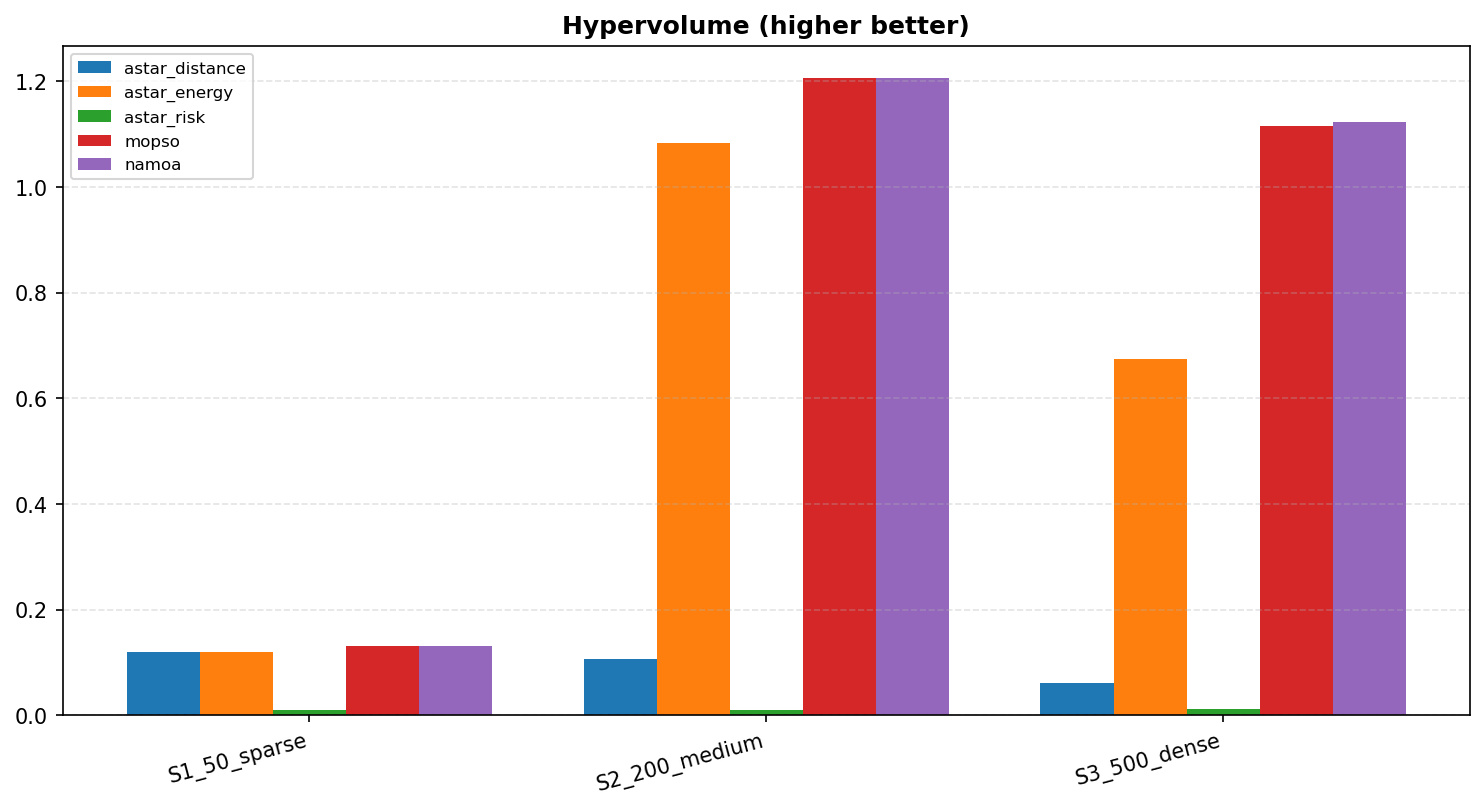
\includegraphics[width=0.62\textwidth]{images/benchmark_hv.jpg}
\caption{Hypervolume per method and scenario (first pass)}\label{fig:bench-hv}
\end{figure}

Exactness has a price. On S3, NAMOA* took 33.8\,s against 4.3\,s for MOPSO, and the
runtime grows quickly with front size. Tier~1 runs once per region and weather window,
not once per mission, so half a minute is acceptable, but it is still the main
performance target for the next pass.

On S2 the HV values of 1.2065 and 1.2061 are too close to claim superiority without
the 30 seeded MOPSO repetitions and a statistical test, which the next pass will run.
The IGD result does not have this problem, since an IGD of zero cannot be beaten.

\subsection{Effect of wind speed and direction}\label{sec:res-wind}

Table~\ref{tab:wind} shows the result of experiment E2.

\begin{table}[!htbp]
\centering
\caption{Effect of wind direction on the S2 front (25\,km/h wind, 35\,km/h gust)}\label{tab:wind}
\footnotesize
\begin{tabular}{|l|r|r|r|r|c|r|}
\hline
\textbf{Wind from} & \textbf{Front} & \textbf{Labels} & \textbf{Min $\boldsymbol{\varepsilon}$} & \textbf{Min $\boldsymbol{\rho}$} & \textbf{Fragile pick $(d, \varepsilon, \rho)$} & \textbf{Distinct}\\
\hline
Calm & 36 & 869 & 24.41 & 0.07 & (26.78, 26.92, 0.11) & 4\\
\hline
0$^\circ$ (N) & 14 & 1019 & 31.01 & 3.24 & (26.16, 32.82, 3.40) & 2\\
\hline
45$^\circ$ (NE) & 6 & 545 & 31.34 & 1.89 & (26.16, 33.63, 1.89) & 2\\
\hline
90$^\circ$ (E) & 11 & 876 & 30.94 & 3.31 & (26.16, 32.75, 3.45) & 2\\
\hline
135$^\circ$ (SE) & 14 & 1100 & 27.13 & 4.27 & (26.16, 29.59, 4.42) & 2\\
\hline
180$^\circ$ (S) & 14 & 989 & 26.18 & 3.24 & (26.16, 27.99, 3.40) & 2\\
\hline
225$^\circ$ (SW) & 6 & 482 & 24.58 & 1.89 & (26.16, 26.87, 1.89) & 2\\
\hline
270$^\circ$ (W) & 11 & 801 & 26.22 & 3.31 & (26.16, 28.03, 3.45) & 2\\
\hline
315$^\circ$ (NW) & 14 & 1084 & 27.21 & 4.27 & (26.16, 29.67, 4.42) & 2\\
\hline
\end{tabular}
\end{table}

The first observation is that direction alone matters a great deal. At the same speed,
the cheapest route on the front needs 24.58 energy units with the wind from the
south-west and 31.34 with it from the north-east, a difference of 27.5\%. A planning
algorithm using wind speed independent of its direction will cost both situations
equally.

The two goals depend on different criteria. When the wind is rotated 180$^\circ$ (from
0$^\circ$ to 180$^\circ$ or from 45$^\circ$ to 225$^\circ$), the lowest risk remains the
same because of the crosswind, which depends only on the wind's axis. Minimum energy
cannot be considered separately from the direction of the wind: the headwind cost is
conditional on the direction of the movement of the drone with respect to the relevant
axis. Both of them derive from Equation~(\ref{eq:hwcw}), which explains why headwind and
crosswind are two separate cases.

The pattern of the front also depends on the state of the wind. In calm conditions, 36
routes are possible; under 8 wind directions, the number of available routes is 6--14,
while the four presets give rise to just two unique routes. The reasoning here is that
in wind, highly crosswind-unfavorable edges become not only expensive but risky, leading
to a coincidence of costs and risks. The most sensitive case -- fragile medical pick --
always provides the safest path in wind, although the energy consumption of the route is
wind-dependent (26.87--33.63). Repeating the run in 15$^\circ$ steps (Figure~\ref{fig:wind-sweep}) gives a
minimum energy of 24.6 to 31.6 units, a 28.5\% swing, with 6 to 15 routes on the front.

\begin{figure}[!htbp]
\centering
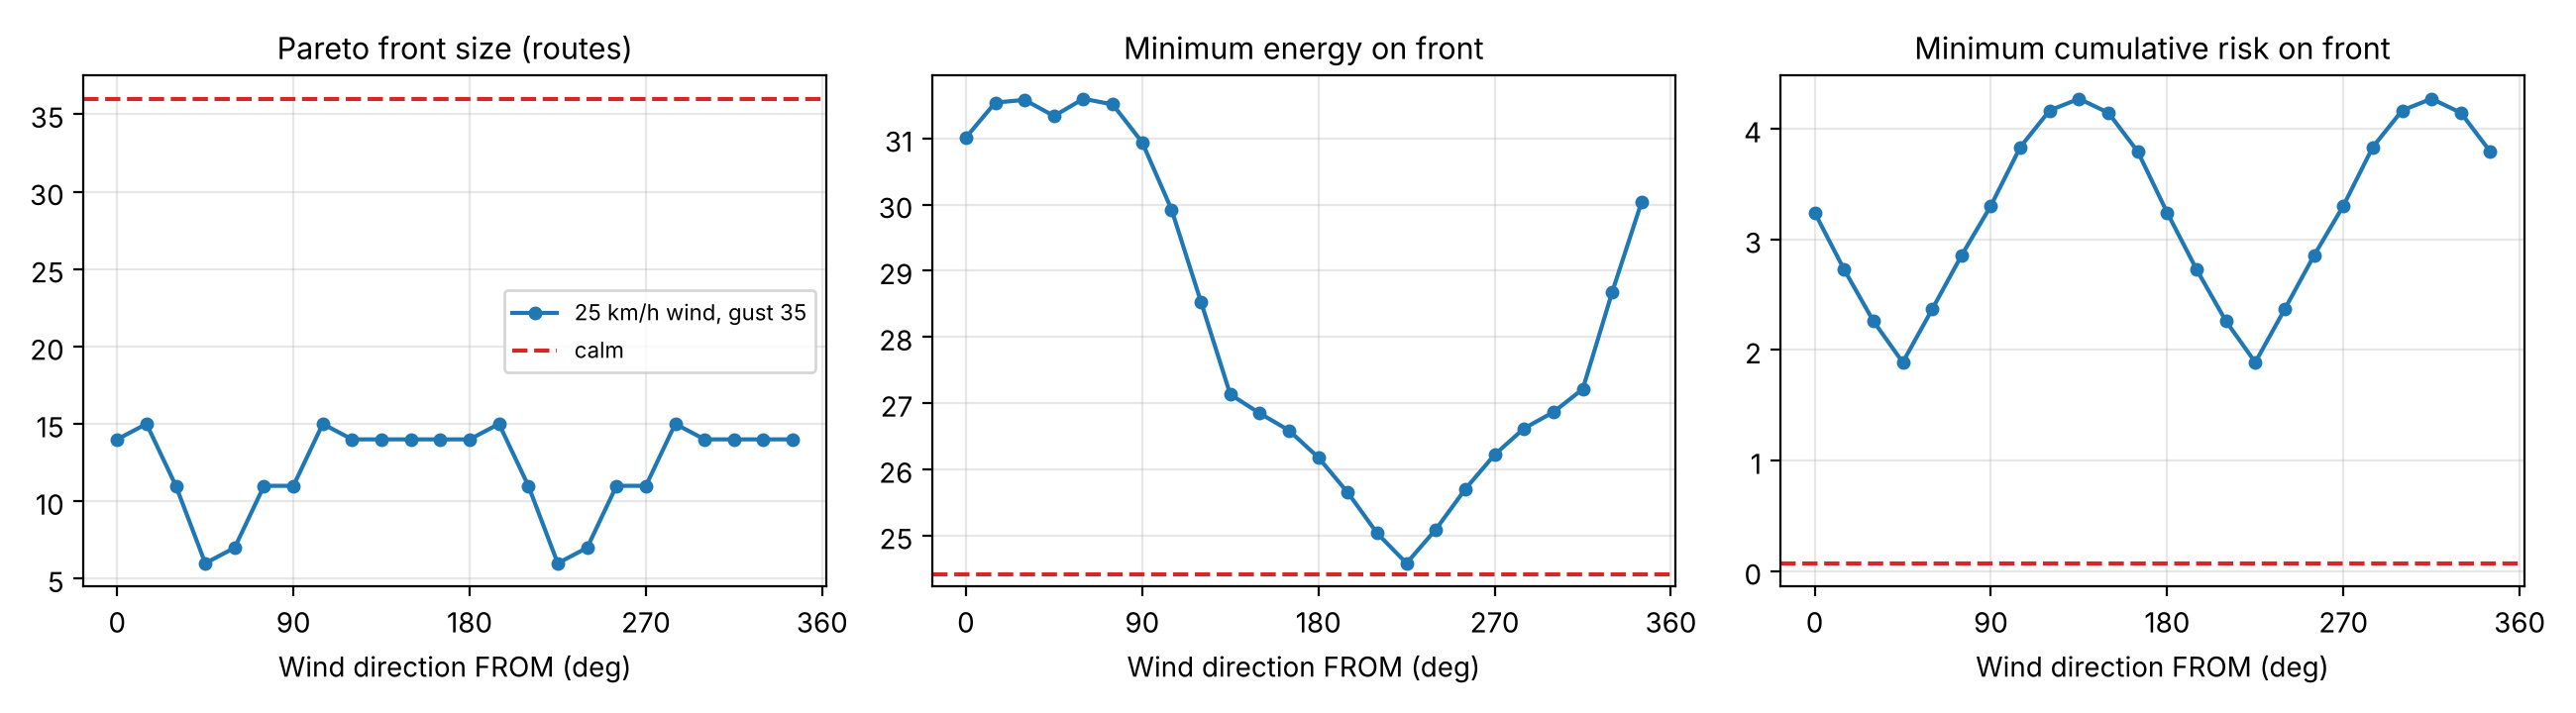
\includegraphics[width=0.9\textwidth]{images/wind_direction_sweep.jpg}
\caption{Front size, minimum energy and minimum risk on S2 as a 25\,km/h wind turns
through 360$^\circ$; the dashed line is calm air}\label{fig:wind-sweep}
\end{figure}

The collapse from four distinct picks to two may be the right answer for a front with
fewer real trade-offs, or a side effect of min-max normalisation on a short front. The
next pass will test both, and the answer may change Tier~2.

\subsection{Directional edge costs}

Table~\ref{tab:dir-edges} gives the result of E3.

\begin{table}[!htbp]
\centering
\caption{Directional edge costs on a flat lattice, 25\,km/h wind from 90$^\circ$}\label{tab:dir-edges}
\small
\begin{tabular}{|l|r|r|r|r|r|r|r|r|}
\hline
\textbf{Edge heading} & 0$^\circ$ & 45$^\circ$ & 90$^\circ$ & 135$^\circ$ & 180$^\circ$ & 225$^\circ$ & 270$^\circ$ & 315$^\circ$\\
\hline
$\varepsilon / d$ & 1.104 & 1.270 & 1.278 & 1.270 & 1.104 & 1.074 & 1.000 & 1.074\\
\hline
$\rho_\mathrm{edge}$ & 0.225 & 0.170 & 0.038 & 0.170 & 0.225 & 0.170 & 0.038 & 0.170\\
\hline
\end{tabular}
\end{table}

Flying east, into the wind, costs 27.8\% more energy per kilometre than flying west,
which costs exactly the distance because a tailwind earns no credit. For north and south
facing edges, the entire crosswind is present, and the risk score is six times that of
east-west edges (0.225 compared to 0.038). The value of 0.038 is only that of the gust
term for east-west edges. Still, the front on the flat lattice has only one route, as the straight diagonal is best for all goals. There is no trade-off resulting from the wind alone.

\subsection{Contribution of each risk layer}\label{sec:perf-ablation}

E4 test results are tabulated in Table~\ref{tab:ablation}. The experiments used fixture layers, so the values show how the layers affect the planner.

\begin{table}[!htbp]
\centering
\caption{Ablation on the 6\,km lattice (fixture layers, 30\,km/h wind from 225$^\circ$)}\label{tab:ablation}
\small
\begin{tabular}{|l|r|r|r|r|r|r|}
\hline
\textbf{Variant} & \textbf{Front} & \textbf{Time (s)} & \textbf{Min $\boldsymbol{\varepsilon}$} & \textbf{Min $\boldsymbol{\rho}$} & \textbf{Max $\boldsymbol{\rho}$} & \textbf{Mean $\boldsymbol{\rho_\mathrm{edge}}$}\\
\hline
All layers & 196 & 11.35 & 8.82 & 8.85 & 13.12 & 0.199\\
\hline
No wind & 205 & 5.38 & 7.84 & 0.10 & 4.24 & 0.061\\
\hline
No terrain & 56 & 1.36 & 8.81 & 8.81 & 13.08 & 0.198\\
\hline
No buildings & 190 & 8.32 & 8.82 & 8.85 & 12.26 & 0.192\\
\hline
\end{tabular}
\end{table}

Wind matters most here: turning it off lowers the mean edge risk
from 0.199 to 0.061, the safest path risk from 8.85 to 0.10, and the minimum energy by
11\%. Terrain, on the other hand, mostly controls how many routes there are. Without
grades there are far fewer distinct trade-offs, 56 routes against 196, because altitude
changes are what separate otherwise similar paths. Buildings raise the top limit of the
risk range.

\subsection{Tier 2 selection}\label{sec:perf-tier2}

Table~\ref{tab:tier2} gives the Tier~2 picks of E5 on the S2 and S3 fronts. The ranks
are the selected route's position on each objective within the front, where 1 is best.

\begin{table}[!htbp]
\centering
\caption{Tier~2 picks on the S2 (16 routes) and S3 (115 routes) fronts}\label{tab:tier2}
\footnotesize
\begin{tabular}{|l|l|r|r|r|r|r|r|l|r|}
\hline
\textbf{Front} & \textbf{Preset} & $\boldsymbol{d}$ & $\boldsymbol{\varepsilon}$ & $\boldsymbol{\rho}$ & \textbf{Rk $d$} & \textbf{Rk $\varepsilon$} & \textbf{Rk $\rho$} & \textbf{Point type} & \textbf{ms}\\
\hline
\multirow{4}{*}{S2} & Fragile medical & 19.45 & 20.94 & 0.69 & 7 & 5 & 10 & non-extreme & 0.030\\
 & Emergency medicine & 19.15 & 20.56 & 0.81 & 3 & 1 & 14 & min-energy & 0.025\\
 & Disaster relief & 19.15 & 20.56 & 0.81 & 3 & 1 & 14 & min-energy & 0.022\\
 & Mixed cargo & 19.22 & 20.66 & 0.75 & 4 & 2 & 13 & non-extreme & 0.023\\
\hline
\multirow{4}{*}{S3} & Fragile medical & 41.02 & 45.86 & 1.92 & 91 & 81 & 25 & non-extreme & 0.144\\
 & Emergency medicine & 37.11 & 44.71 & 6.56 & 22 & 26 & 94 & non-extreme & 0.140\\
 & Disaster relief & 37.52 & 44.27 & 5.63 & 28 & 1 & 88 & min-energy & 0.136\\
 & Mixed cargo & 39.90 & 45.06 & 2.74 & 84 & 59 & 32 & non-extreme & 0.136\\
\hline
\end{tabular}
\end{table}

On the 115-route S3 front, the four presets take four separate routes, three of which are represented by non-extreme points. Disaster relief uses the minimum energy path, consistent with its dominant weight.

The emergency medicine preset deserves a special consideration. It is merely the
22nd shortest route, yet it is just 1.9\% longer than the shortest route in the front.
While the distance is the key factor in the setting of its weights, it is not the only
one; therefore, the utility function sacrifices some distance for smaller risk. A single
objective planner cannot do that kind of tradeoff, and a fixed weights planner would
make the same tradeoff for each payload.

The fragile medical and emergency routes show the gap between Tier~2 options. The fragile route is 10.5\% longer than the emergency one
(41.02 versus 37.11), and it has 71\% less risk (1.92 versus 6.56). It ranks 25th out of
115 on risk instead of 1st, because both distance and energy coefficients are still positive and the more cautious paths are much longer.
Mixed cargo is in an intermediate position with respect to all criteria, as expected from its balanced weights. Selections on S3
took about 0.14\,ms, against a target of one second.

On the smaller S2 front, emergency medicine and disaster relief take the same minimal energy path, as in the wind example: small fronts leave Tier~2 fewer paths.

Figure~\ref{fig:osm-routes} shows the four presets on a 2\,km lattice (11-route front) with
OpenStreetMap roads drawn underneath for reference. The fragile medical and mixed cargo
presets take a slightly longer path (2.6\,km) with a cumulative risk of 1.57, while
emergency medicine and disaster relief take 2.5\,km paths with risks of 1.88 and 1.89.

\begin{figure}[!htbp]
\centering
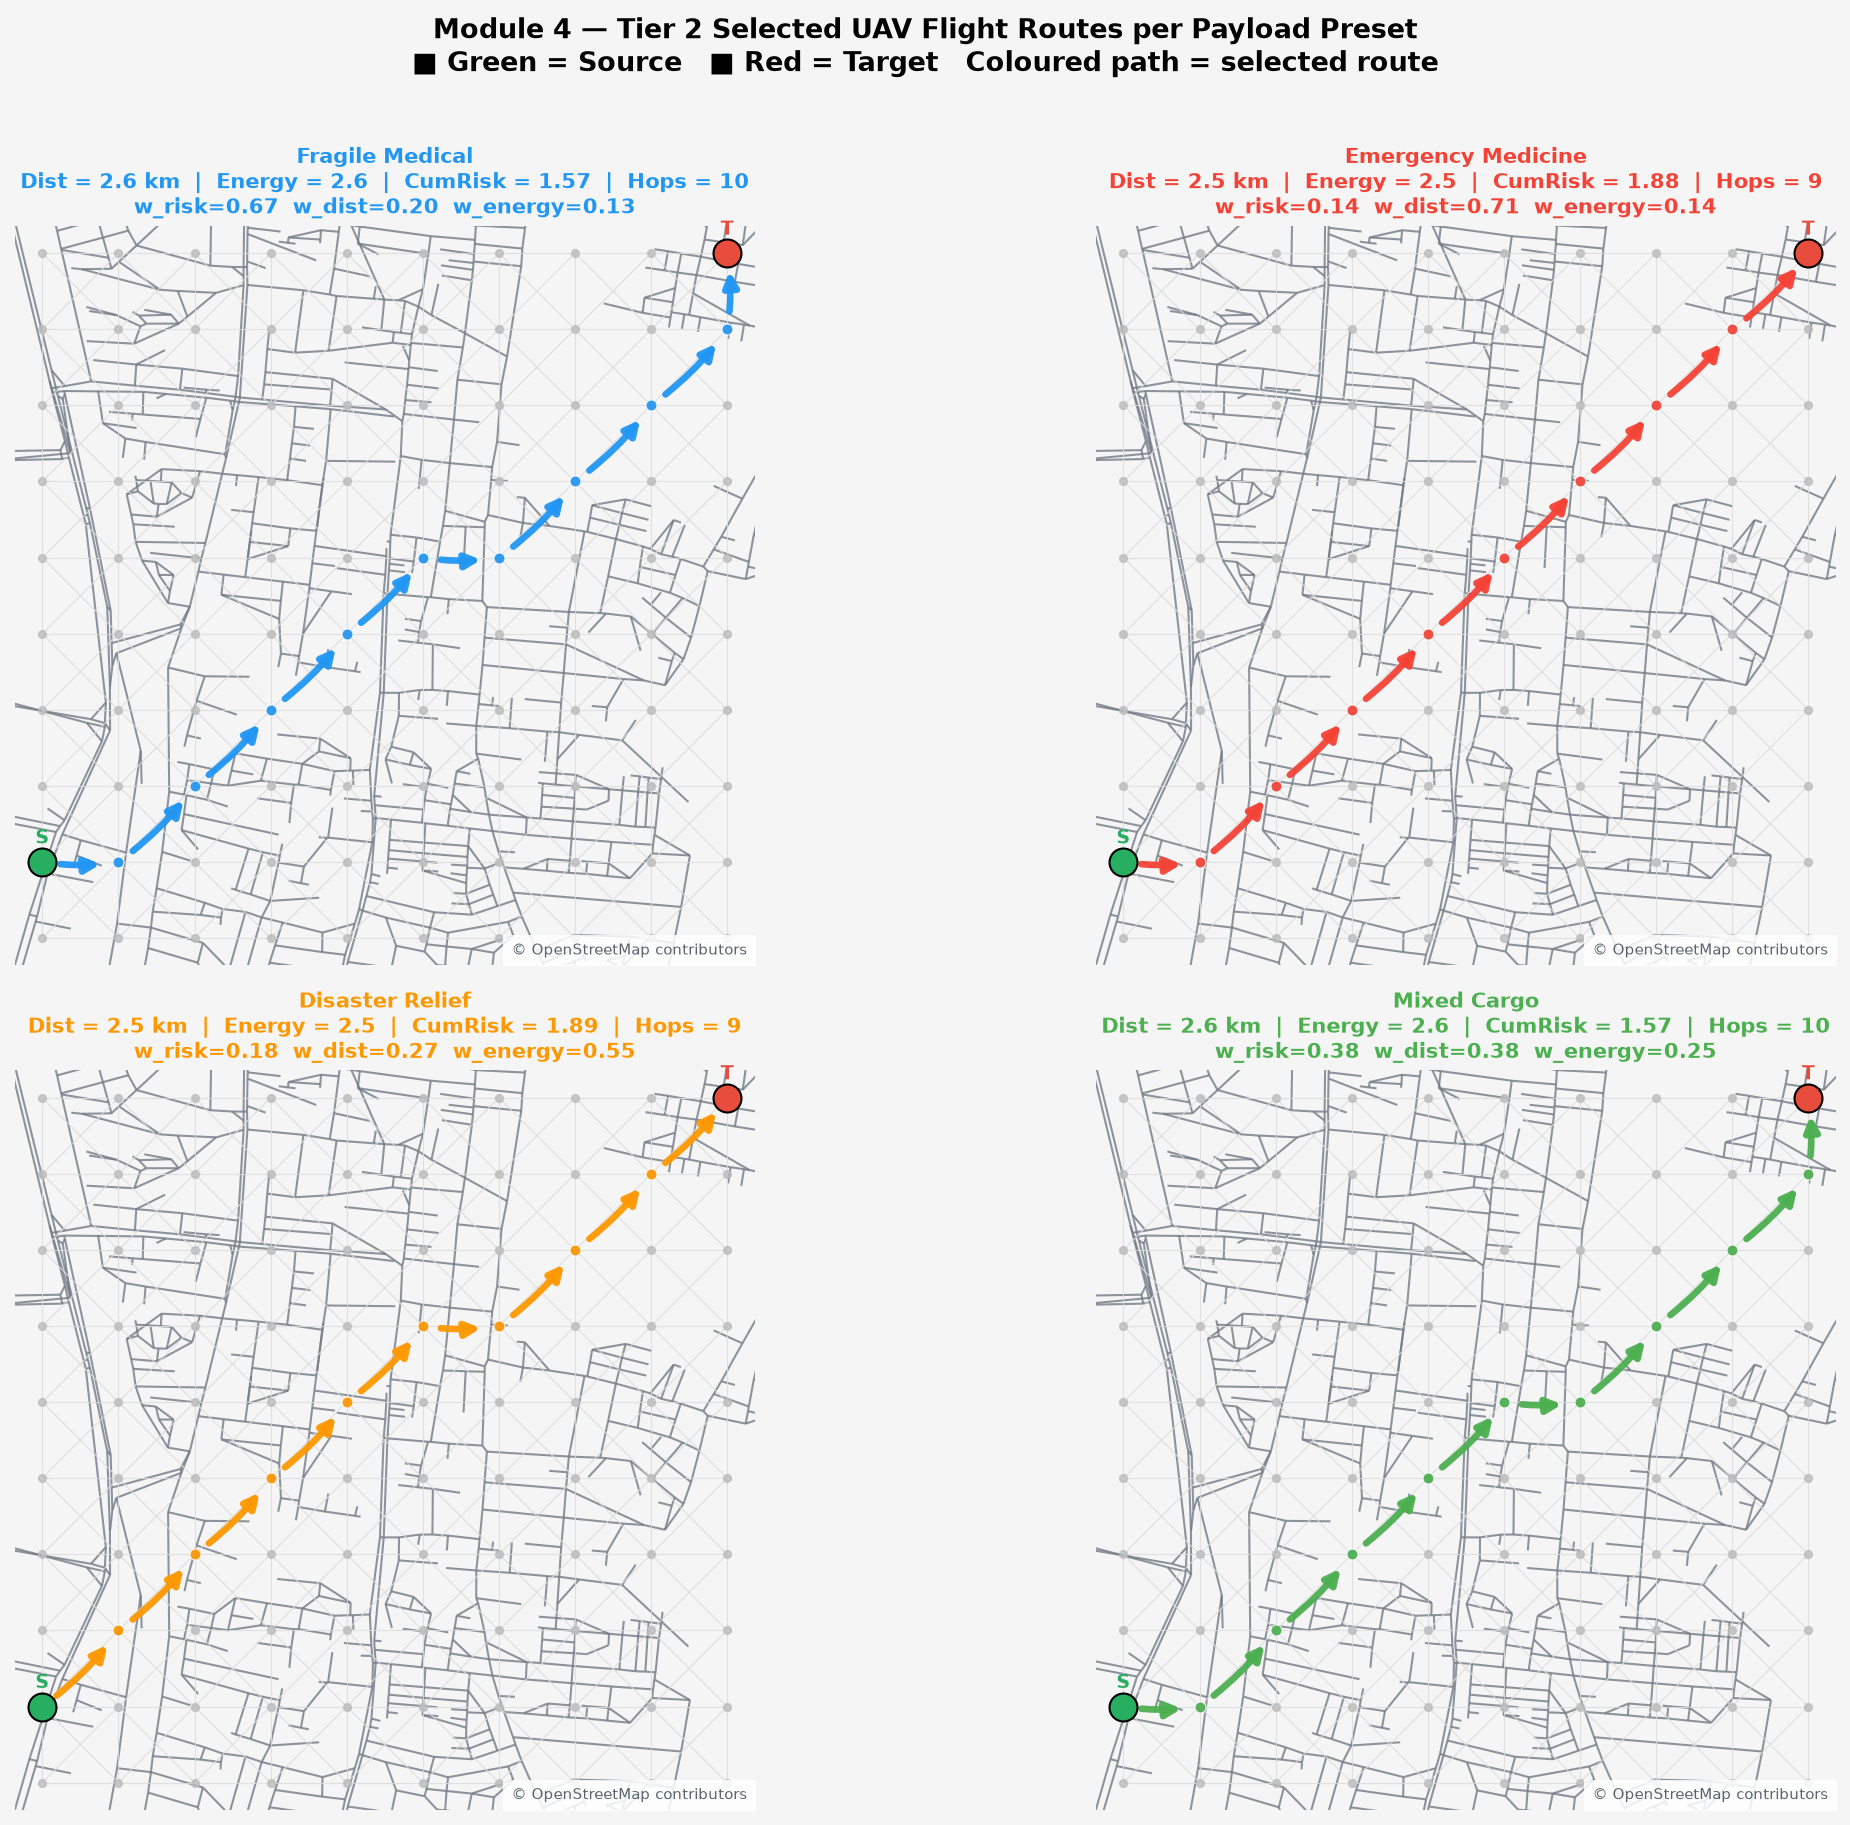
\includegraphics[width=0.48\textwidth]{images/osm_module4_routes_on_graph.jpg}
\caption{Tier~2 routes for the four presets on the 2\,km lattice}\label{fig:osm-routes}
\end{figure}

The first monotonicity check reported 660 violations on the smallest benchmark, but it
had compared selections across scenarios; grouped by scenario, the count is zero.

\subsection{Simulation results}

In E6 the SITL mission runner flew planner missions against ArduCopter SITL. Mission
upload, read-back, the switch to AUTO, the landing and the disarm all succeeded. The
cross-track root-mean-square error between the flown and planned tracks was
0.11--0.13\,m, and the landing offset from the destination pad was 0.01--0.02\,m. These
numbers show that the mission chain from Tier~2 to the autopilot is correct, including
the altitude frame, which is easy to get wrong over uneven terrain.

Figure~\ref{fig:sitl} shows a Tier~2 mission flown in AUTO inside the Gazebo city world,
with the MAVProxy console on the left and the mission in QGroundControl on the right.
The Gazebo world has no wind yet, so logged comparisons across wind cases are planned
for the next pass.

\begin{figure}[!htbp]
\centering
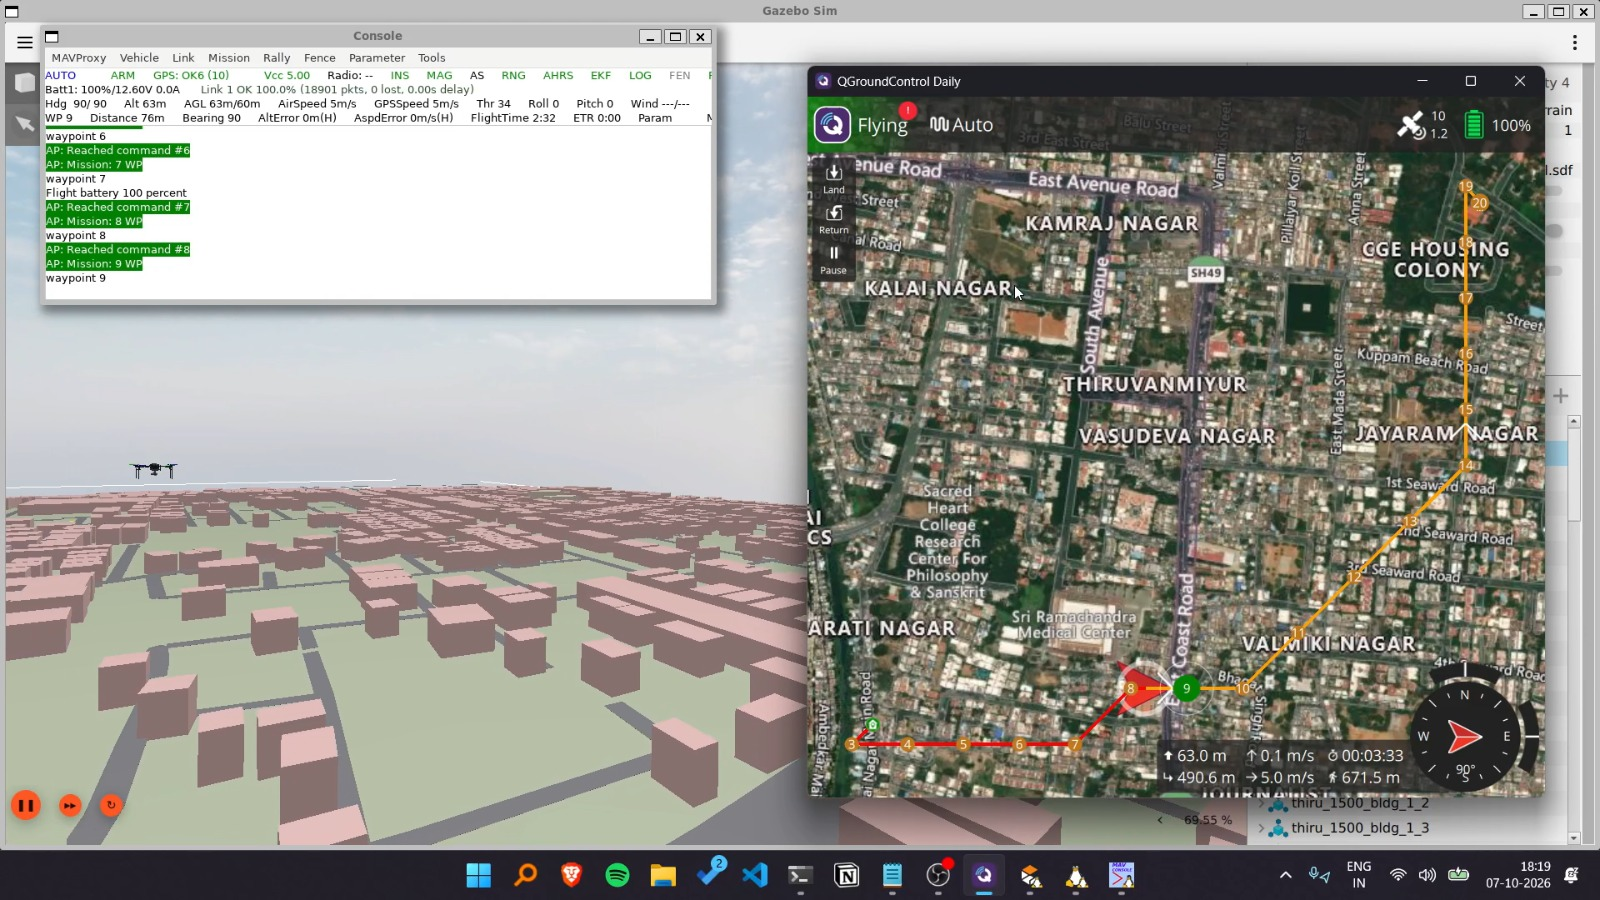
\includegraphics[width=0.6\textwidth]{images/sitl_gazebo_screenshot.jpg}
\caption{Gazebo Harmonic and ArduPilot SITL flying an uploaded Tier~2 mission in AUTO:
MAVProxy console (left), QGroundControl mission view (right)}\label{fig:sitl}
\end{figure}

\subsection{Comparison with existing work}

Table~\ref{tab:compare} compares the system with the planners reviewed in
Chapter~\ref{cha:lit}.

\begin{footnotesize}
\begin{longtable}{|P{1.8cm}|P{2.4cm}|P{2.1cm}|P{2.1cm}|P{2.3cm}|P{2.9cm}|}
\caption{Comparison with the reviewed planners}\label{tab:compare}\\
\hline
\textbf{Property} & \textbf{Chokkalingam and Ganesan~\cite{r1}} & \textbf{Ren et al.~\cite{r3}} & \textbf{Deng et al.~\cite{r11}} & \textbf{Tsoutsouras et al.~\cite{r10}} & \textbf{This work}\\
\hline
\endfirsthead
\hline
\textbf{Property} & \textbf{Chokkalingam and Ganesan~\cite{r1}} & \textbf{Ren et al.~\cite{r3}} & \textbf{Deng et al.~\cite{r11}} & \textbf{Tsoutsouras et al.~\cite{r10}} & \textbf{This work}\\
\hline
\endhead
Front construction & POPSO, stochastic & CDNSGA-II, stochastic & MS-INSGA2, stochastic & None; one trajectory & NAMOA*, exact and deterministic\\
\hline
Objectives & Length, energy, safety, obstacle penalty, weather factor & Distance, safety & Length, collision risk, smoothness & Deadline misses under energy and mass limits & Distance, energy, risk (11 components)\\
\hline
Final route selection & Weighted sum, weights set per mission & Crowding distance ($k$ nearest) & Not discussed & Not applicable & Utility from payload tags, argmax over the full front\\
\hline
Payload in selection & No & No & No & Mass in the power model only & Fragility, weight class, urgency, priority\\
\hline
Wind & Speed-only factor, uniform & Not modelled & Future work & Not modelled & Headwind and crosswind per edge, gust, shear, weather gate\\
\hline
Front reuse & Re-run per mission & Re-run per mission & Re-run per task & Not applicable & Stored front with drift-based refresh\\
\hline
\end{longtable}
\end{footnotesize}

The comparison is qualitative, as their datasets and code are not public; the next pass
scores their selection rules on our fronts (Section~\ref{sec:m5}).
 % EXPERIMENTAL RESULTS AND PERFORMANCE ANALYSIS
% Chapter 5

\chapter{SOCIAL IMPACT AND SUSTAINABILITY}\label{cha:social}

\section{SOCIAL IMPACT}

Drone delivery helps most the people who live far from a hospital or are cut off by an
emergency. Rural healthcare logistics considerations would be in cases where there was a
need for blood or an antivenom in a clinic, a town surrounded by floods, or regular
delivery of samples from a hospital to a laboratory in one day. Similar services already exist, such as Zipline drones in Rwanda~\cite{r16} and hospital samples flights in Switzerland~\cite{r12}. The suggested method adds a way for
each flight to adapt to the particular cargo, where urgent antivenom would fly through
the shortest path while fragile cargo would use another path. This advantage is important since there might be a situation where no specialists in
planning will be available. The launch of a drone from a district hospital or a relief
camp will be conducted either by a nurse or volunteers instead of a specialist in
planning. This person needs only to provide four simple answers about the cargo
characteristics (frangible, weight, urgency, and importance), after which all other
decisions will be made automatically.

Underneath, there are people who do not want the drone to fly above their heads. Every
edge cost considers aspects such as population, restricted areas, water distance, and
building distance. All nodes that exceed the statutory limit are disregarded, and
adverse weather conditions make it impossible for flights if there are storms, rainfall,
poor visibility, and high winds. There is no way that the planner will go through a
crowded market just to save a few seconds.

All decisions made at Tier~2 level are saved along with the corresponding tags, weights,
route, and any HOLD reason. The fragility tag
is a precaution and has not been shown to protect anything~\cite{r13,r14,r15}. Until
proper risk weights are set, the derived risk values will act as relative rankings of
the routes rather than probabilities of harm. Phase~II outdoor flights will follow the
Drone Rules, 2021~\cite{r21}.

\section{SUSTAINABILITY}

For the short-distance flights of light payloads, an electric-powered drone may be
substituted for van or motorcycle transport without exhaust emission during travel. The
planner helps in two major ways. Firstly, its energy goal considers the wind direction,
which alone changed the energy of the cheapest route by 27.5\%, implying that headwinds
may be avoided. Secondly, the payload weight label gives more weight to energy criteria
for heavy payloads. Flights whose battery energy is exhausted to less than the 20\%
reserve level are excluded, thereby assuring both the success of the flight and battery
longevity.

The computational demand is low as well. Tier~1 runs on an ordinary laptop CPU with no
GPU or cloud service, once per region and weather window. Tier~2 takes a fraction of a
millisecond and can run on a Raspberry Pi on board. Everything the system depends on is open data or open-source software, so there are no licence fees.
 % SOCIAL IMPACT AND SUSTAINABILITY
% Chapter 6

\chapter{CONCLUSION AND FUTURE WORK}\label{cha:conclusion}

\section{CONCLUSION}

This project set out to let the payload decide the route. Existing multi-objective UAV
planners build good Pareto fronts and then choose from them with a rule that knows
nothing about the cargo, or with weights an expert re-tunes for every mission. We
separated the two problems. Tier~1 builds an exact NAMOA* front over a
three-dimensional, wind-aware airspace lattice once per region and weather window, and
stores it until it goes stale. Tier~2 turns four payload
tags into objective weights with an explicit formula, scores every route on the front
and returns the best one, or a HOLD when the weather or the battery rules the mission
out. The chosen route has been flown in SITL and in a Gazebo city world.

The preliminary results have been quite encouraging, but there are still some important
observations to make. First, the Tier~1 front was exact for each of the benchmarks, while MOPSO managed to discover 38 routes
out of 115 on the biggest one. On that front the four reference payloads received four
different routes, three of them non-extreme, in about 0.14\,ms each. Secondly, when only the wind direction was varied at constant speed,
the energy consumed on the route that had the lowest cost changed by 27.5\%. The results
of the SITL simulations showed that the drone stayed within 0.13\,m RMS of the planned
trajectory. However, there were a number of flaws found as well. In a steady wind the front
shrank and the presets fell onto two routes; MOPSO ran at reduced settings; the ablation
used fixture data; and the risk weights and battery constants are still placeholders.

\section{FUTURE WORK}

The following experiment conducts the full benchmark (four graphs, nine wind cases,
MOPSO set to use 100 particles, 200 iterations, and 30 runs) with stats for each run and
significance test. Density tags and monotonicity classification need fixing, and our
goal is to find out the reason for Pareto collapse in constant wind case by testing
other normalization and weight multipliers. Ablation and Tier~2 experiments will be
performed again but using real map data, and then Tier~2 will be tested against
crowding distance, knee point, shortest route, and fixed weights for all 225 tag
combinations. There are two flaws in the dashboard that are not fixed yet, and Tier~1
needs better performance in large graphs. Simulation involves putting the Gazebo world
through wind, tuning the battery model according to the class of load it carries, and
running the pre-defined setup for all different wind conditions with full flight logs
recorded. For Phase~II, the system switches to using an F450 quadcopter with the Pixhawk and a
companion computer called Raspberry Pi~5 and a servo for releasing the payload. The
Tier~2 system runs on the drone, and outdoor testing will involve checking the extent to
which it stays on course and the time between entering tags and starting the mission.
Following this, the two-tier system can be further expanded to include multiple drones
having a common front, performing multi-drop delivery missions, or in-flight
re-planning of routes based on the changing weather.
 % CONCLUSION AND FUTURE WORK

\clearpage
\addtotoc{REFERENCES}
% APA style, alphabetical by first author; numbers follow this order.
\begin{spacing}{1.15}
\small
\begin{thebibliography}{99}
\setlength{\itemsep}{2pt}

\bibitem{r23}
ArduPilot Development Team. (2026). \textit{ArduPilot software in the loop (SITL) simulator}. \url{https://ardupilot.org/dev/docs/sitl-simulator-software-in-the-loop.html}

\bibitem{r12}
Avionics International. (2019, August 8). \textit{Drone delivery crash in Switzerland raises safety concerns as UPS forms subsidiary}. \url{https://www.aviationtoday.com/2019/08/08/drone-delivery-crash-in-switzerland-raises-safety-concerns/}

\bibitem{r4}
Boeing, G. (2017). OSMnx: New methods for acquiring, constructing, analyzing, and visualizing complex street networks. \textit{Computers, Environment and Urban Systems}, \textit{65}, 126--139. \url{https://doi.org/10.1016/j.compenvurbsys.2017.05.004}

\bibitem{r1}
Chokkalingam, K., \& Ganesan, R. (2026). Dynamic parameter adaptation in Pareto-optimal particle swarm optimization for efficient UAV path planning. \textit{RAIRO -- Operations Research}, \textit{60}(1), 281--305. \url{https://doi.org/10.1051/ro/2025159}

\bibitem{r6}
Coello Coello, C. A., Toscano Pulido, G., \& Salazar Lechuga, M. (2004). Handling multiple objectives with particle swarm optimization. \textit{IEEE Transactions on Evolutionary Computation}, \textit{8}(3), 256--279. \url{https://doi.org/10.1109/TEVC.2004.826067}

\bibitem{r8}
Deb, K., Pratap, A., Agarwal, S., \& Meyarivan, T. (2002). A fast and elitist multiobjective genetic algorithm: NSGA-II. \textit{IEEE Transactions on Evolutionary Computation}, \textit{6}(2), 182--197. \url{https://doi.org/10.1109/4235.996017}

\bibitem{r11}
Deng, J., Zhang, H., Feng, D., Yu, Z., \& Liu, Z. (2026). Multi-objective UAV trajectory planning algorithm based on the hybrid MS-INSGA2 strategy. \textit{Journal of King Saud University -- Computer and Information Sciences}, \textit{38}, Article 562. \url{https://doi.org/10.1007/s44443-026-00930-0}

\bibitem{r5}
Hagberg, A. A., Schult, D. A., \& Swart, P. J. (2008). Exploring network structure, dynamics, and function using NetworkX. In \textit{Proceedings of the 7th Python in Science Conference (SciPy 2008)} (pp. 11--15). \url{https://doi.org/10.25080/TCWV9851}

\bibitem{r16}
IEEE Spectrum. (2019). \textit{In the air with Zipline's medical delivery drones}. \url{https://spectrum.ieee.org/in-the-air-with-ziplines-medical-delivery-drones}

\bibitem{r22}
Joint Authorities for Rulemaking of Unmanned Systems. (2019). \textit{JARUS guidelines on specific operations risk assessment (SORA)} (JAR-DEL-WG6-D.04, Edition 2.0).

\bibitem{r17}
Mandow, L., \& P\'{e}rez de la Cruz, J. L. (2010). Multiobjective A* search with consistent heuristics. \textit{Journal of the ACM}, \textit{57}(5), Article 27. \url{https://doi.org/10.1145/1754399.1754400}

\bibitem{r7}
Meier, L., et al. (2013). \textit{MAVLink: Micro air vehicle communication protocol}. \url{https://mavlink.io}

\bibitem{r21}
Ministry of Civil Aviation, Government of India. (2021). \textit{The Drone Rules, 2021} (G.S.R. 589(E)). Gazette of India.

\bibitem{r13}
Oakey, A., Waters, T., Zhu, W., Royall, P. G., Cherrett, T., Courtney, P., Majoe, D., \& Jelev, N. (2021). Quantifying the effects of vibration on medicines in transit caused by fixed-wing and multi-copter drones. \textit{Drones}, \textit{5}(1), 22. \url{https://doi.org/10.3390/drones5010022}

\bibitem{r20}
Open-Meteo. (2026). \textit{Free weather API and elevation API}. \url{https://open-meteo.com}

\bibitem{r24}
Open Robotics. (2023). \textit{Gazebo Harmonic}. \url{https://gazebosim.org}

\bibitem{r19}
Peterson, E. W., \& Hennessey, J. P. (1978). On the use of power laws for estimates of wind power potential. \textit{Journal of Applied Meteorology}, \textit{17}(3), 390--394. \url{https://doi.org/10.1175/1520-0450(1978)017<0390:OTUOPL>2.0.CO;2}

\bibitem{r3}
Ren, Q., Yao, Y., Yang, G., \& Zhou, X. (2019). Multi-objective path planning for UAV in the urban environment based on CDNSGA-II. In \textit{Proceedings of the IEEE International Conference on Service-Oriented System Engineering (SOSE)}. \url{https://doi.org/10.1109/SOSE.2019.00059}

\bibitem{r15}
Stierlin, N., Loertscher, F., Renz, H., Risch, L., \& Risch, M. (2024). Preanalytic integrity of blood samples in uncrewed aerial vehicle (UAV) medical transport: A comparative study. \textit{Drones}, \textit{8}(9), 517. \url{https://doi.org/10.3390/drones8090517}

\bibitem{r14}
Theobald, K., Zhu, W., Waters, T., Cherrett, T., Oakey, A., \& Royall, P. G. (2023). Stability of medicines transported by cargo drones: Investigating the effects of vibration from multi-stage flight. \textit{Drones}, \textit{7}(11), 658. \url{https://doi.org/10.3390/drones7110658}

\bibitem{r10}
Tsoutsouras, V., Story, J., \& Stanley-Marbell, P. (2020). \textit{Payload-mass-aware trajectory planning on multi-user autonomous unmanned aerial vehicles} (arXiv:2001.02531). arXiv. \url{https://doi.org/10.48550/arXiv.2001.02531}

\bibitem{r18}
Zitzler, E., \& Thiele, L. (1999). Multiobjective evolutionary algorithms: A comparative case study and the strength Pareto approach. \textit{IEEE Transactions on Evolutionary Computation}, \textit{3}(4), 257--271. \url{https://doi.org/10.1109/4235.797969}

\end{thebibliography}
\end{spacing}

% Appendices

\appendix

\chapter{CONFIGURATION PARAMETERS}\label{app:params}

All tunable constants live in \texttt{config.py}. Table~\ref{tab:params} lists the main
parameters of the airspace graph and cost model, and Table~\ref{tab:params2} those of the
front store and Tier~2. Values marked provisional are placeholders that will be replaced
by calibrated values.

\begin{table}[!htbp]
\centering
\caption{Main airspace graph and cost model parameters}\label{tab:params}
\small
\begin{tabular}{|P{5.0cm}|P{2.6cm}|P{6.6cm}|}
\hline
\textbf{Parameter} & \textbf{Value} & \textbf{Meaning}\\
\hline
\texttt{BOX\_M}, \texttt{LATTICE\_SPACING\_M} & 6000\,m, 200\,m & Lattice extent and spacing\\
\hline
\texttt{H\_CRUISE\_AGL}, \texttt{CLEARANCE} & 60\,m, 15\,m & Cruise height, margin above roofs\\
\hline
\texttt{H\_MAX\_AGL} & 120\,m & Legal ceiling above ground\\
\hline
\texttt{V\_CRUISE\_KMH} & 36\,km/h & Airspeed used in the wind terms\\
\hline
\texttt{BETA\_HEAD}, \texttt{BETA\_CROSS} & 0.40, 0.15 & Headwind and crosswind energy coefficients\\
\hline
\texttt{V\_MAX\_SAFE\_KMH}, \texttt{K\_GUST} & 40\,km/h, 0.5 & Wind risk saturation speed, gust weight\\
\hline
\texttt{ALPHA\_SHEAR} & 0.25 & Power-law wind shear exponent\\
\hline
\texttt{EDGE\_SAMPLE\_STEP\_M} & 25\,m & Sampling step along each edge\\
\hline
\texttt{NFZ\_SOFT\_LAMBDA\_M} & 150\,m & Decay length of the no-fly buffer\\
\hline
\texttt{NO\_GO\_GUST\_KMH} & 45\,km/h & Gust limit of the weather gate (provisional)\\
\hline
\texttt{RISK\_WEIGHTS} & Table~\ref{tab:risk} & Weights of the eleven risk components (uncalibrated)\\
\hline
\end{tabular}
\end{table}

\begin{table}[!htbp]
\centering
\caption{Front store and Tier~2 parameters}\label{tab:params2}
\small
\begin{tabular}{|P{5.0cm}|P{3.4cm}|P{5.8cm}|}
\hline
\textbf{Parameter} & \textbf{Value} & \textbf{Meaning}\\
\hline
Front validity window & 3\,h & Front expires after this time\\
\hline
Wind speed drift & 10\,km/h & Rebuild when wind speed moves more than this\\
\hline
Wind direction drift & 45$^\circ$ (wind $>$ 10\,km/h) & Rebuild when wind turns more than this\\
\hline
Gust drift & 15\,km/h & Rebuild when gust moves more than this\\
\hline
Tier~1 expansion cap & 200,000 (S1/S2/S3: 80k, 180k, 260k) & Guards against runaway search\\
\hline
Payload masses $m_W$ & 0.25, 0.5, 1.0\,kg & Nominal mass of weight classes 1, 2, 3\\
\hline
$m_\mathrm{uav}$, battery, reserve & 1.5\,kg, 74\,Wh, 20\% & Airframe mass and battery (provisional)\\
\hline
$k_\mathrm{cal}$ & 6\,Wh per unit & Energy proxy to watt-hours (provisional)\\
\hline
Priority threshold & $P_\mathrm{lvl} \geq 4$ & Dominant weight amplified by 10\%\\
\hline
\end{tabular}
\end{table}

\FloatBarrier
\flowchapter{AUTOMATED TEST SUITES}\label{app:tests}

Both code bases have offline unit-test suites that need no network and no API key.
The planner suite has about 220 tests and the simulation suite 45.
Table~\ref{tab:tests} lists what they check.

\begin{small}
\begin{longtable}{|P{5.6cm}|P{8.6cm}|}
\caption{Test suites and what they verify}\label{tab:tests}\\
\hline
\textbf{Test file} & \textbf{What it checks}\\
\hline
\endfirsthead
\hline
\textbf{Test file} & \textbf{What it checks}\\
\hline
\endhead
\texttt{test\_wind.py} & Headwind sign (wind from 90$^\circ$ is a headwind for an east-bound edge), crosswind, power-law shear, hourly row selection\\
\hline
\texttt{test\_lattice.py} & Lattice size, 8-neighbour edges, east-bound edges cost more than west-bound edges under an east wind\\
\hline
\texttt{test\_terrain.py} & DEM provider chain and cache, node altitude rule, every node within 120\,m above ground\\
\hline
\texttt{test\_risk.py} & Risk components in $[0,1]$, restricted-zone node and edge removal, soft buffer, weather gate\\
\hline
\texttt{test\_tier1\_front.py} & NAMOA* front equals a brute-force front over all simple paths on a small graph; no route dominates another; every path valid\\
\hline
\texttt{test\_store.py} & Reuse, expiry, graph-hash change, each drift threshold, identity check\\
\hline
\texttt{test\_tier2\_payload.py}, \texttt{test\_tier2\_hardening.py} & Weight formula, amplification, non-extreme pick for mixed cargo on a stored lattice front, monotonicity, validation errors, latency under 1\,s, battery HOLD\\
\hline
\texttt{test\_evaluation\_metrics.py} & HV, IGD and spread on hand-computed cases; alignment score; competing pickers\\
\hline
\texttt{test\_mission\_export.py} & QGC WPL~110 round trip, collinear merge, frame~3 altitude relative to home\\
\hline
\texttt{test\_ablation.py}, \texttt{test\_overpass.py}, \texttt{test\_dotenv.py}, \texttt{test\_dashboard\_helpers.py} & Ablation smoke run, Overpass retry and parsing, key loading, dashboard helpers\\
\hline
\texttt{Simulation/tests/*} & Bundle loading and frames, clearance checker, mission export (take-off, route, land), world builder geometry\\
\hline
\end{longtable}
\end{small}

\chapter{CODE ORGANISATION}\label{app:code}

The planner is written in Python as flat scripts, one file per module, plus a
configuration file, an environment-data file and entry-point scripts. The simulation
lives in a separate folder and imports the planner modules through the Python path.
Every tunable constant (region, flight heights, wind coefficients, risk weights,
battery and mass values, drift thresholds, Overpass endpoints) lives in one file,
\texttt{config.py}, so an experiment changes a value in one place. API keys are read
from a \texttt{.env} file by the entry-point scripts only, so the test suites never need
a key or a network connection. Table~\ref{tab:files} maps the source files to the
modules.

\begin{table}[!htbp]
\centering
\caption{Source files and the modules they implement}\label{tab:files}
\small
\begin{tabular}{|P{5.2cm}|P{1.4cm}|P{7.6cm}|}
\hline
\textbf{File} & \textbf{Module} & \textbf{Role}\\
\hline
\texttt{config.py} & all & Every tunable constant\\
\hline
\texttt{env\_data.py} & 1 & Weather, DEM providers, OSM layers, spatial indexes, key loader\\
\hline
\texttt{overpass\_client.py} & 1 & Multi-endpoint Overpass fetch with retry\\
\hline
\texttt{module1\_graph\_builder.py} & 1 & Synthetic and lattice builders, cost pipeline\\
\hline
\texttt{module2\_tier1\_moastar.py} & 2 & NAMOA* engine, dominance helpers, thinning\\
\hline
\texttt{pareto\_store.py} & 2 & Front store, graph hash, drift, region runs\\
\hline
\texttt{module3\_baselines.py} & 3 & A* variants, weighted-sum A*, MOPSO\\
\hline
\texttt{module4\_tier2\_payload.py} & 4 & Weight bridge, selector, feasibility, export\\
\hline
\texttt{module5\_evaluation.py} & 5 & HV, IGD, spread, Tier~2 evidence, sweep\\
\hline
\texttt{run\_benchmarks.py}, \texttt{run\_ablation.py} & 5 & Benchmark and ablation runners\\
\hline
\texttt{mission\_export.py}, \texttt{dashboard.py} & 6 & QGC WPL~110 export, operator interface\\
\hline
\texttt{run\_demo\_syn.py}, \texttt{run\_demo\_osm.py} & 1--4 & End-to-end demonstrations with figures\\
\hline
\texttt{Simulation/*.py} & 7 & Bundle, clearance, world, mission, runner, logger, evaluator\\
\hline
\end{tabular}
\end{table}



\end{spacing}
\end{document}
